% Options for packages loaded elsewhere
\PassOptionsToPackage{unicode}{hyperref}
\PassOptionsToPackage{hyphens}{url}
\PassOptionsToPackage{dvipsnames,svgnames,x11names}{xcolor}
%
\documentclass[
  letterpaper,
  DIV=11,
  numbers=noendperiod]{scrartcl}

\usepackage{amsmath,amssymb}
\usepackage{iftex}
\ifPDFTeX
  \usepackage[T1]{fontenc}
  \usepackage[utf8]{inputenc}
  \usepackage{textcomp} % provide euro and other symbols
\else % if luatex or xetex
  \usepackage{unicode-math}
  \defaultfontfeatures{Scale=MatchLowercase}
  \defaultfontfeatures[\rmfamily]{Ligatures=TeX,Scale=1}
\fi
\usepackage{lmodern}
\ifPDFTeX\else  
    % xetex/luatex font selection
\fi
% Use upquote if available, for straight quotes in verbatim environments
\IfFileExists{upquote.sty}{\usepackage{upquote}}{}
\IfFileExists{microtype.sty}{% use microtype if available
  \usepackage[]{microtype}
  \UseMicrotypeSet[protrusion]{basicmath} % disable protrusion for tt fonts
}{}
\makeatletter
\@ifundefined{KOMAClassName}{% if non-KOMA class
  \IfFileExists{parskip.sty}{%
    \usepackage{parskip}
  }{% else
    \setlength{\parindent}{0pt}
    \setlength{\parskip}{6pt plus 2pt minus 1pt}}
}{% if KOMA class
  \KOMAoptions{parskip=half}}
\makeatother
\usepackage{xcolor}
\usepackage[top=2.5cm, bottom=2.5cm, left=3cm, right=3cm]{geometry}
\setlength{\emergencystretch}{3em} % prevent overfull lines
\setcounter{secnumdepth}{5}
% Make \paragraph and \subparagraph free-standing
\makeatletter
\ifx\paragraph\undefined\else
  \let\oldparagraph\paragraph
  \renewcommand{\paragraph}{
    \@ifstar
      \xxxParagraphStar
      \xxxParagraphNoStar
  }
  \newcommand{\xxxParagraphStar}[1]{\oldparagraph*{#1}\mbox{}}
  \newcommand{\xxxParagraphNoStar}[1]{\oldparagraph{#1}\mbox{}}
\fi
\ifx\subparagraph\undefined\else
  \let\oldsubparagraph\subparagraph
  \renewcommand{\subparagraph}{
    \@ifstar
      \xxxSubParagraphStar
      \xxxSubParagraphNoStar
  }
  \newcommand{\xxxSubParagraphStar}[1]{\oldsubparagraph*{#1}\mbox{}}
  \newcommand{\xxxSubParagraphNoStar}[1]{\oldsubparagraph{#1}\mbox{}}
\fi
\makeatother

\usepackage{color}
\usepackage{fancyvrb}
\newcommand{\VerbBar}{|}
\newcommand{\VERB}{\Verb[commandchars=\\\{\}]}
\DefineVerbatimEnvironment{Highlighting}{Verbatim}{commandchars=\\\{\}}
% Add ',fontsize=\small' for more characters per line
\usepackage{framed}
\definecolor{shadecolor}{RGB}{241,243,245}
\newenvironment{Shaded}{\begin{snugshade}}{\end{snugshade}}
\newcommand{\AlertTok}[1]{\textcolor[rgb]{0.68,0.00,0.00}{#1}}
\newcommand{\AnnotationTok}[1]{\textcolor[rgb]{0.37,0.37,0.37}{#1}}
\newcommand{\AttributeTok}[1]{\textcolor[rgb]{0.40,0.45,0.13}{#1}}
\newcommand{\BaseNTok}[1]{\textcolor[rgb]{0.68,0.00,0.00}{#1}}
\newcommand{\BuiltInTok}[1]{\textcolor[rgb]{0.00,0.23,0.31}{#1}}
\newcommand{\CharTok}[1]{\textcolor[rgb]{0.13,0.47,0.30}{#1}}
\newcommand{\CommentTok}[1]{\textcolor[rgb]{0.37,0.37,0.37}{#1}}
\newcommand{\CommentVarTok}[1]{\textcolor[rgb]{0.37,0.37,0.37}{\textit{#1}}}
\newcommand{\ConstantTok}[1]{\textcolor[rgb]{0.56,0.35,0.01}{#1}}
\newcommand{\ControlFlowTok}[1]{\textcolor[rgb]{0.00,0.23,0.31}{\textbf{#1}}}
\newcommand{\DataTypeTok}[1]{\textcolor[rgb]{0.68,0.00,0.00}{#1}}
\newcommand{\DecValTok}[1]{\textcolor[rgb]{0.68,0.00,0.00}{#1}}
\newcommand{\DocumentationTok}[1]{\textcolor[rgb]{0.37,0.37,0.37}{\textit{#1}}}
\newcommand{\ErrorTok}[1]{\textcolor[rgb]{0.68,0.00,0.00}{#1}}
\newcommand{\ExtensionTok}[1]{\textcolor[rgb]{0.00,0.23,0.31}{#1}}
\newcommand{\FloatTok}[1]{\textcolor[rgb]{0.68,0.00,0.00}{#1}}
\newcommand{\FunctionTok}[1]{\textcolor[rgb]{0.28,0.35,0.67}{#1}}
\newcommand{\ImportTok}[1]{\textcolor[rgb]{0.00,0.46,0.62}{#1}}
\newcommand{\InformationTok}[1]{\textcolor[rgb]{0.37,0.37,0.37}{#1}}
\newcommand{\KeywordTok}[1]{\textcolor[rgb]{0.00,0.23,0.31}{\textbf{#1}}}
\newcommand{\NormalTok}[1]{\textcolor[rgb]{0.00,0.23,0.31}{#1}}
\newcommand{\OperatorTok}[1]{\textcolor[rgb]{0.37,0.37,0.37}{#1}}
\newcommand{\OtherTok}[1]{\textcolor[rgb]{0.00,0.23,0.31}{#1}}
\newcommand{\PreprocessorTok}[1]{\textcolor[rgb]{0.68,0.00,0.00}{#1}}
\newcommand{\RegionMarkerTok}[1]{\textcolor[rgb]{0.00,0.23,0.31}{#1}}
\newcommand{\SpecialCharTok}[1]{\textcolor[rgb]{0.37,0.37,0.37}{#1}}
\newcommand{\SpecialStringTok}[1]{\textcolor[rgb]{0.13,0.47,0.30}{#1}}
\newcommand{\StringTok}[1]{\textcolor[rgb]{0.13,0.47,0.30}{#1}}
\newcommand{\VariableTok}[1]{\textcolor[rgb]{0.07,0.07,0.07}{#1}}
\newcommand{\VerbatimStringTok}[1]{\textcolor[rgb]{0.13,0.47,0.30}{#1}}
\newcommand{\WarningTok}[1]{\textcolor[rgb]{0.37,0.37,0.37}{\textit{#1}}}

\providecommand{\tightlist}{%
  \setlength{\itemsep}{0pt}\setlength{\parskip}{0pt}}\usepackage{longtable,booktabs,array}
\usepackage{calc} % for calculating minipage widths
% Correct order of tables after \paragraph or \subparagraph
\usepackage{etoolbox}
\makeatletter
\patchcmd\longtable{\par}{\if@noskipsec\mbox{}\fi\par}{}{}
\makeatother
% Allow footnotes in longtable head/foot
\IfFileExists{footnotehyper.sty}{\usepackage{footnotehyper}}{\usepackage{footnote}}
\makesavenoteenv{longtable}
\usepackage{graphicx}
\makeatletter
\newsavebox\pandoc@box
\newcommand*\pandocbounded[1]{% scales image to fit in text height/width
  \sbox\pandoc@box{#1}%
  \Gscale@div\@tempa{\textheight}{\dimexpr\ht\pandoc@box+\dp\pandoc@box\relax}%
  \Gscale@div\@tempb{\linewidth}{\wd\pandoc@box}%
  \ifdim\@tempb\p@<\@tempa\p@\let\@tempa\@tempb\fi% select the smaller of both
  \ifdim\@tempa\p@<\p@\scalebox{\@tempa}{\usebox\pandoc@box}%
  \else\usebox{\pandoc@box}%
  \fi%
}
% Set default figure placement to htbp
\def\fps@figure{htbp}
\makeatother

\usepackage{fancyhdr}
\pagestyle{fancy}
\fancyhf{}
\fancyhead[L]{Asociación entre Edad Avanzada y Diagnóstico de Alzheimer}
\fancyhead[R]{Matías Elier Labraña Abarca}
\fancyfoot[C]{\thepage}
\usepackage{etoolbox}
\AtBeginEnvironment{Shaded}{\small}  % Cambia \small por \footnotesize o \scriptsize si quieres más pequeño
\usepackage{booktabs}
\usepackage{longtable}
\usepackage{array}
\usepackage{multirow}
\usepackage{wrapfig}
\usepackage{float}
\usepackage{colortbl}
\usepackage{pdflscape}
\usepackage{tabu}
\usepackage{threeparttable}
\usepackage{threeparttablex}
\usepackage[normalem]{ulem}
\usepackage{makecell}
\usepackage{xcolor}
\KOMAoption{captions}{tableheading}
\makeatletter
\@ifpackageloaded{caption}{}{\usepackage{caption}}
\AtBeginDocument{%
\ifdefined\contentsname
  \renewcommand*\contentsname{Table of contents}
\else
  \newcommand\contentsname{Table of contents}
\fi
\ifdefined\listfigurename
  \renewcommand*\listfigurename{List of Figures}
\else
  \newcommand\listfigurename{List of Figures}
\fi
\ifdefined\listtablename
  \renewcommand*\listtablename{List of Tables}
\else
  \newcommand\listtablename{List of Tables}
\fi
\ifdefined\figurename
  \renewcommand*\figurename{Figure}
\else
  \newcommand\figurename{Figure}
\fi
\ifdefined\tablename
  \renewcommand*\tablename{Table}
\else
  \newcommand\tablename{Table}
\fi
}
\@ifpackageloaded{float}{}{\usepackage{float}}
\floatstyle{ruled}
\@ifundefined{c@chapter}{\newfloat{codelisting}{h}{lop}}{\newfloat{codelisting}{h}{lop}[chapter]}
\floatname{codelisting}{Listing}
\newcommand*\listoflistings{\listof{codelisting}{List of Listings}}
\makeatother
\makeatletter
\makeatother
\makeatletter
\@ifpackageloaded{caption}{}{\usepackage{caption}}
\@ifpackageloaded{subcaption}{}{\usepackage{subcaption}}
\makeatother
\makeatletter
\@ifpackageloaded{tcolorbox}{}{\usepackage[skins,breakable]{tcolorbox}}
\makeatother
\makeatletter
\@ifundefined{shadecolor}{\definecolor{shadecolor}{rgb}{.97, .97, .97}}{}
\makeatother
\makeatletter
\makeatother
\makeatletter
\ifdefined\Shaded\renewenvironment{Shaded}{\begin{tcolorbox}[interior hidden, breakable, frame hidden, enhanced, boxrule=0pt, sharp corners]}{\end{tcolorbox}}\fi
\makeatother

\usepackage{bookmark}

\IfFileExists{xurl.sty}{\usepackage{xurl}}{} % add URL line breaks if available
\urlstyle{same} % disable monospaced font for URLs
\hypersetup{
  pdftitle={Asociación entre Datos Médicos y Diagnóstico de Alzheimer},
  pdfauthor={Matías Elier Labraña Abarca},
  colorlinks=true,
  linkcolor={blue},
  filecolor={Maroon},
  citecolor={Blue},
  urlcolor={Blue},
  pdfcreator={LaTeX via pandoc}}


\title{Asociación entre Datos Médicos y Diagnóstico de Alzheimer}
\usepackage{etoolbox}
\makeatletter
\providecommand{\subtitle}[1]{% add subtitle to \maketitle
  \apptocmd{\@title}{\par {\large #1 \par}}{}{}
}
\makeatother
\subtitle{Análisis Estadístico de Datos Clínicos con Enfoque Tidyverse}
\author{Matías Elier Labraña Abarca}
\date{Invalid Date}

\begin{document}
\maketitle

\renewcommand*\contentsname{Table of contents}
{
\hypersetup{linkcolor=}
\setcounter{tocdepth}{3}
\tableofcontents
}

\pagebreak

\section{Introducción}\label{introducciuxf3n}

Este estudio tiene como objetivo identificar los factores clínicos y
demográficos asociados al diagnóstico de la enfermedad de Alzheimer a
partir del análisis del conjunto de datos \emph{Alzheimer's Disease
Data} (Kaggle). Se emplea un enfoque sistemático basado en el ecosistema
\textbf{Tidyverse}, el cual facilita tanto la limpieza de los datos como
la exploración de relaciones significativas entre variables como edad,
nivel educativo, antecedentes familiares y puntuaciones cognitivas
(MMSE).

\subsubsection{Objetivos del análisis}\label{objetivos-del-anuxe1lisis}

\begin{itemize}
\item
  \textbf{Preprocesamiento de datos} utilizando las herramientas del
  Tidyverse para garantizar su calidad y consistencia.

  \textbf{Análisis exploratorio de datos (AED)} enfocado en la
  identificación de patrones y relaciones entre variables relevantes.

  \textbf{Desarrollo de una función reproducible} para automatizar el
  análisis y facilitar su aplicación a futuros datasets similares.
\end{itemize}

\section{Definición del Problema}\label{definiciuxf3n-del-problema}

\paragraph{Problema de
Investigación}\label{problema-de-investigaciuxf3n}

La enfermedad de Alzheimer es una condición neurodegenerativa progresiva
que afecta significativamente la calidad de vida de quienes la padecen.
La identificación de factores de riesgo tempranos constituye un desafío
clave en el ámbito de la salud pública y la investigación biomédica, ya
que permitiría diseñar estrategias preventivas más eficaces y
personalizadas.

\paragraph{Objetivo General}\label{objetivo-general}

El objetivo de este estudio es explorar las relaciones existentes entre
características demográficas, factores clínicos y el diagnóstico de la
enfermedad de Alzheimer, evaluando además la factibilidad de desarrollar
un modelo predictivo basado en dichas variables.

\paragraph{Variables Clave}\label{variables-clave}

\begin{itemize}
\item
  \textbf{Variables Cuantitativas}:

  \begin{itemize}
  \item
    \textbf{Age (Edad)}: Edad del paciente en años. Se plantea la
    hipótesis de que una mayor edad está asociada con un riesgo más
    elevado de desarrollar Alzheimer
  \item
    \textbf{MMSE (Mini-Mental State Examination)}: Puntaje obtenido en
    la evaluación cognitiva. Se espera que puntuaciones más bajas se
    correlacionen con un diagnóstico de Alzheimer.
  \end{itemize}

  \textbf{Variables Cualitativas}:

  \begin{itemize}
  \item
    \textbf{FamilyHistoryAlzheimers}: Antecedentes familiares de
    Alzheimer (sí/no). Se plantea que contar con antecedentes familiares
    incrementa el riesgo de desarrollar la enfermedad.
  \item
    \textbf{EducationLevel}: Nivel educativo alcanzado. Se investigará
    la posible relación entre los niveles educativos (bajo, medio, alto)
    y el diagnóstico de Alzheimer.
  \end{itemize}
\end{itemize}

\pagebreak

\section{Datos y Metodología}\label{datos-y-metodologuxeda}

\subsubsection{Descripción del
Dataset}\label{descripciuxf3n-del-dataset}

En primer lugar, se listan los archivos con extensión \textbf{.csv} en
el directorio de trabajo actual, con el propósito de verificar la
presencia del archivo requerido: \texttt{alzheimers\_disease\_data.csv}.
Esta verificación inicial es fundamental para evitar errores durante el
proceso de carga.

A continuación, se procede a cargar el dataset utilizando la función
\textbf{\texttt{read\_csv}} del paquete \textbf{readr}, que forma parte
del ecosistema \textbf{tidyverse}. Se implementa un manejo de errores
robusto para asegurar que la carga se realice de manera exitosa y
detener el proceso en caso de fallos, garantizando la confiabilidad de
los datos desde la etapa inicial.

Una vez completada la carga, se inspeccionan las dimensiones del
dataset, el número de filas y columnas para obtener un panorama general
de su tamaño. Posteriormente, se efectúa una revisión preliminar de
valores ausentes (\textbf{NA}) en todas las columnas, generando un
resumen con la cantidad de datos faltantes por variable. Esta
información es crucial para detectar problemas de calidad de datos que
deberán abordarse en etapas posteriores.

Finalmente, se presenta un listado de las principales variables
utilizadas en el análisis, con una breve descripción de cada una,
incluyendo su tipo (cuantitativa o cualitativa) y su relevancia en el
estudio.

\begin{Shaded}
\begin{Highlighting}[]
\FunctionTok{print}\NormalTok{(}\FunctionTok{list.files}\NormalTok{(}\AttributeTok{pattern =} \StringTok{"*.csv"}\NormalTok{))}
\end{Highlighting}
\end{Shaded}

\begin{verbatim}
[1] "alzheimers_disease_data.csv"
\end{verbatim}

\begin{Shaded}
\begin{Highlighting}[]
\CommentTok{\# Asigna el nombre del .CSV a una variable}
\NormalTok{archivo }\OtherTok{\textless{}{-}} \StringTok{"alzheimers\_disease\_data.csv"} 

\CommentTok{\# Inicializar una bandera para rastrear el éxito de la carga del archivo.}
\NormalTok{carga\_exitosa }\OtherTok{\textless{}{-}} \ConstantTok{TRUE}

\CommentTok{\# Intentar cargar el archivo CSV utilizando readr::read\_csv.}
\CommentTok{\# Se incluye manejo de errores para capturar problemas durante la carga.}
\NormalTok{alzheimer\_raw }\OtherTok{\textless{}{-}} \FunctionTok{tryCatch}\NormalTok{(}
\NormalTok{  \{}
    \CommentTok{\# show\_col\_types = FALSE evita mensajes sobre los tipos de columna.}
\NormalTok{    readr}\SpecialCharTok{::}\FunctionTok{read\_csv}\NormalTok{(archivo, }\AttributeTok{show\_col\_types =} \ConstantTok{FALSE}\NormalTok{)}
\NormalTok{  \},}
  \AttributeTok{error =} \ControlFlowTok{function}\NormalTok{(captura\_error) \{}
    \CommentTok{\# En caso de error, mostrar un mensaje descriptivo.}
    \FunctionTok{message}\NormalTok{(}\StringTok{"Error al cargar el archivo: "}\NormalTok{, captura\_error}\SpecialCharTok{$}\NormalTok{message)}
    \CommentTok{\# Actualizar la bandera para indicar que la carga falló.}
\NormalTok{    carga\_exitosa }\OtherTok{\textless{}\textless{}{-}} \ConstantTok{FALSE} \CommentTok{\# \textless{}\textless{}{-} para modificar la variable en el entorno global del chunk.}
    \CommentTok{\# Devolver NULL como resultado de la operación fallida.}
    \ConstantTok{NULL}
\NormalTok{  \}}
\NormalTok{)}

\CommentTok{\# Verificar si la carga fue exitosa y el objeto de datos no es NULL.}
\ControlFlowTok{if}\NormalTok{ (carga\_exitosa }\SpecialCharTok{\&\&} \SpecialCharTok{!}\FunctionTok{is.null}\NormalTok{(alzheimer\_raw)) \{}
  \FunctionTok{message}\NormalTok{(}\StringTok{"Carga exitosa del archivo."}\NormalTok{)}
\NormalTok{\} }\ControlFlowTok{else}\NormalTok{ \{}
  \FunctionTok{message}\NormalTok{(}\StringTok{"No se pudo cargar el archivo. Verifica la ruta y el nombre."}\NormalTok{)}
  \CommentTok{\# Detener la ejecución del documento si la carga del archivo falla.}
\NormalTok{  knitr}\SpecialCharTok{::}\FunctionTok{knit\_exit}\NormalTok{() }
\NormalTok{\}}
\end{Highlighting}
\end{Shaded}

\begin{Shaded}
\begin{Highlighting}[]
\CommentTok{\# Verificar que el dataset \textquotesingle{}alzheimer\_raw\textquotesingle{} exista y no sea NULL antes de proceder.}
\ControlFlowTok{if}\NormalTok{ (}\FunctionTok{exists}\NormalTok{(}\StringTok{"alzheimer\_raw"}\NormalTok{) }\SpecialCharTok{\&\&} \SpecialCharTok{!}\FunctionTok{is.null}\NormalTok{(alzheimer\_raw)) \{}
  \CommentTok{\# Imprimir las dimensiones del dataset.}
  \FunctionTok{cat}\NormalTok{(}\FunctionTok{paste0}\NormalTok{(}\StringTok{"El dataset original contiene "}\NormalTok{, }\FunctionTok{nrow}\NormalTok{(alzheimer\_raw), }\StringTok{" filas y "}\NormalTok{,}
      \FunctionTok{ncol}\NormalTok{(alzheimer\_raw), }\StringTok{" columnas.}\SpecialCharTok{\textbackslash{}n}\StringTok{"}\NormalTok{))}
\NormalTok{\}}
\end{Highlighting}
\end{Shaded}

\begin{verbatim}
El dataset original contiene 2149 filas y 35 columnas.
\end{verbatim}

\subsection{Procesamiento}\label{procesamiento}

Esta sección se centra en la preparación y limpieza del dataset original
(\texttt{alzheimer\_raw}). A continuación, se ejecutan pasos clave para
garantizar la calidad de los datos y su correcta tipificación antes de
los análisis posteriores. Primero, se realiza una revisión exhaustiva de
los valores ausentes y se documentan las variables que presentan datos
faltantes. Luego, se transforman variables categóricas y numéricas a sus
formatos adecuados, facilitando la consistencia en las etapas de
análisis y modelado. Finalmente, se ajusta el dataset para excluir
columnas irrelevantes o identificadores únicos, obteniendo un conjunto
final de datos (\texttt{alzheimer\_analisis}) listo para las fases de
exploración y modelado.

\subsubsection{Limpieza Inicial}\label{limpieza-inicial}

\begin{Shaded}
\begin{Highlighting}[]
\CommentTok{\# Revisión inicial de valores ausentes (NA).}
\CommentTok{\# Verificar que el dataset \textquotesingle{}alzheimer\_raw\textquotesingle{} exista y no sea NULL.}
\ControlFlowTok{if}\NormalTok{ (}\FunctionTok{exists}\NormalTok{(}\StringTok{"alzheimer\_raw"}\NormalTok{) }\SpecialCharTok{\&\&} \SpecialCharTok{!}\FunctionTok{is.null}\NormalTok{(alzheimer\_raw)) \{}
  \CommentTok{\# Calcular la cantidad de valores NA por columna.}
\NormalTok{  missing\_values\_summary }\OtherTok{\textless{}{-}}\NormalTok{ alzheimer\_raw }\SpecialCharTok{\%\textgreater{}\%}
    \FunctionTok{summarise}\NormalTok{(}
      \CommentTok{\# Aplicar la función sum(is.na(.)) a todas las columnas.}
      \FunctionTok{across}\NormalTok{(}
        \FunctionTok{everything}\NormalTok{(),       }
        \SpecialCharTok{\textasciitilde{}} \FunctionTok{sum}\NormalTok{(}\FunctionTok{is.na}\NormalTok{(.))     }
\NormalTok{      )}
\NormalTok{    ) }\SpecialCharTok{\%\textgreater{}\%}
    \CommentTok{\# Convertir el resumen de formato ancho a largo para facilitar el filtrado y visualización.}
    \FunctionTok{pivot\_longer}\NormalTok{(}
      \FunctionTok{everything}\NormalTok{(),             }
      \AttributeTok{names\_to =} \StringTok{"columna"}\NormalTok{,     }
      \AttributeTok{values\_to =} \StringTok{"cantidad\_na"} 
\NormalTok{    ) }\SpecialCharTok{\%\textgreater{}\%}
    \CommentTok{\# Filtrar para mostrar solo las columnas que tienen al menos un valor NA.}
    \FunctionTok{filter}\NormalTok{(cantidad\_na }\SpecialCharTok{\textgreater{}} \DecValTok{0}\NormalTok{)   }

  \CommentTok{\# Visualización de los resultados del conteo de NAs.}
  \CommentTok{\# Si se encontraron columnas con valores ausentes, mostrar un resumen.}
  \ControlFlowTok{if}\NormalTok{ (}\FunctionTok{nrow}\NormalTok{(missing\_values\_summary) }\SpecialCharTok{\textgreater{}} \DecValTok{0}\NormalTok{) \{}
    \FunctionTok{cat}\NormalTok{(}\StringTok{"Se identificaron valores ausentes en las siguientes columnas:}\SpecialCharTok{\textbackslash{}n}\StringTok{"}\NormalTok{)}
    \CommentTok{\# Imprimir la tabla de valores perdidos usando kable para un formato legible.}
    \FunctionTok{print}\NormalTok{(knitr}\SpecialCharTok{::}\FunctionTok{kable}\NormalTok{(}
\NormalTok{      missing\_values\_summary,}
      \AttributeTok{caption =} \StringTok{"Resumen de Valores Perdidos Iniciales"}
\NormalTok{    ))}
    \FunctionTok{cat}\NormalTok{(}\StringTok{"Estos valores serán considerados en etapas posteriores del análisis.}\SpecialCharTok{\textbackslash{}n}\StringTok{"}\NormalTok{)}
\NormalTok{  \} }\ControlFlowTok{else}\NormalTok{ \{}
    \CommentTok{\# Si no se encontraron NAs, informar al usuario.}
    \FunctionTok{cat}\NormalTok{(}\StringTok{"No se encontraron valores perdidos en una revisión inicial del dataset.}\SpecialCharTok{\textbackslash{}n}\StringTok{"}\NormalTok{)}
\NormalTok{  \}}
\NormalTok{\}}
\end{Highlighting}
\end{Shaded}

\begin{verbatim}
No se encontraron valores perdidos en una revisión inicial del dataset.
\end{verbatim}

\begin{Shaded}
\begin{Highlighting}[]
\CommentTok{\# Descripción breve de las variables clave (reiteración de la sección de Objetivos).}
\FunctionTok{cat}\NormalTok{(}\StringTok{"}\SpecialCharTok{\textbackslash{}n}\StringTok{Variables principales del estudio (reiteración):}\SpecialCharTok{\textbackslash{}n}\StringTok{"}\NormalTok{)}
\end{Highlighting}
\end{Shaded}

\begin{verbatim}

Variables principales del estudio (reiteración):
\end{verbatim}

\begin{Shaded}
\begin{Highlighting}[]
\FunctionTok{cat}\NormalTok{(}\StringTok{"{-} Age (Numérica): Edad del paciente en años.}\SpecialCharTok{\textbackslash{}n}\StringTok{"}\NormalTok{)}
\end{Highlighting}
\end{Shaded}

\begin{verbatim}
- Age (Numérica): Edad del paciente en años.
\end{verbatim}

\begin{Shaded}
\begin{Highlighting}[]
\FunctionTok{cat}\NormalTok{(}\StringTok{"{-} MMSE (Numérica): Puntaje Mini{-}Mental State Examination.}\SpecialCharTok{\textbackslash{}n}\StringTok{"}\NormalTok{)}
\end{Highlighting}
\end{Shaded}

\begin{verbatim}
- MMSE (Numérica): Puntaje Mini-Mental State Examination.
\end{verbatim}

\begin{Shaded}
\begin{Highlighting}[]
\FunctionTok{cat}\NormalTok{(}\StringTok{"{-} FamilyHistoryAlzheimers (Categórica Binaria): Antecedentes familiares.}\SpecialCharTok{\textbackslash{}n}\StringTok{"}\NormalTok{)}
\end{Highlighting}
\end{Shaded}

\begin{verbatim}
- FamilyHistoryAlzheimers (Categórica Binaria): Antecedentes familiares.
\end{verbatim}

\begin{Shaded}
\begin{Highlighting}[]
\FunctionTok{cat}\NormalTok{(}\StringTok{"{-} EducationLevel (Categórica Ordinal): Nivel educativo.}\SpecialCharTok{\textbackslash{}n}\StringTok{"}\NormalTok{)}
\end{Highlighting}
\end{Shaded}

\begin{verbatim}
- EducationLevel (Categórica Ordinal): Nivel educativo.
\end{verbatim}

\begin{Shaded}
\begin{Highlighting}[]
\FunctionTok{cat}\NormalTok{(}\StringTok{"{-} Diagnosis (Categórica Binaria): Diagnóstico de Alzheimer (1 = Sí, 0 = No).}\SpecialCharTok{\textbackslash{}n}\StringTok{"}\NormalTok{)}
\end{Highlighting}
\end{Shaded}

\begin{verbatim}
- Diagnosis (Categórica Binaria): Diagnóstico de Alzheimer (1 = Sí, 0 = No).
\end{verbatim}

\subsubsection{Trasformación de
Variable}\label{trasformaciuxf3n-de-variable}

\begin{Shaded}
\begin{Highlighting}[]
\CommentTok{\# Verificar que el dataset \textquotesingle{}alzheimer\_raw\textquotesingle{} exista y no sea NULL.}
\ControlFlowTok{if}\NormalTok{ (}\FunctionTok{exists}\NormalTok{(}\StringTok{"alzheimer\_raw"}\NormalTok{) }\SpecialCharTok{\&\&} \SpecialCharTok{!}\FunctionTok{is.null}\NormalTok{(alzheimer\_raw)) \{}
 
  \CommentTok{\# Lista de columnas a convertir en factor.}
\NormalTok{  cols\_to\_factor }\OtherTok{\textless{}{-}} \FunctionTok{c}\NormalTok{(}
  \StringTok{"BehavioralProblems"}\NormalTok{,       }\StringTok{"CardiovascularDisease"}\NormalTok{,}
  \StringTok{"Confusion"}\NormalTok{,                }\StringTok{"Depression"}\NormalTok{,}
  \StringTok{"Diabetes"}\NormalTok{,                 }\StringTok{"DifficultyCompletingTasks"}\NormalTok{,}
  \StringTok{"Disorientation"}\NormalTok{,           }\StringTok{"EducationLevel"}\NormalTok{,}
  \StringTok{"Ethnicity"}\NormalTok{,                }\StringTok{"FamilyHistoryAlzheimers"}\NormalTok{,}
  \StringTok{"Forgetfulness"}\NormalTok{,            }\StringTok{"Gender"}\NormalTok{,}
  \StringTok{"HeadInjury"}\NormalTok{,               }\StringTok{"Hypertension"}\NormalTok{,}
  \StringTok{"MemoryComplaints"}\NormalTok{,         }\StringTok{"PersonalityChanges"}\NormalTok{,}
  \StringTok{"Smoking"}
\NormalTok{)}
  
\CommentTok{\# Crear el dataset \textquotesingle{}alzheimer\textquotesingle{} aplicando las transformaciones.}
\NormalTok{alzheimer }\OtherTok{\textless{}{-}}\NormalTok{ alzheimer\_raw }\SpecialCharTok{\%\textgreater{}\%}
  \CommentTok{\# Convertir las columnas en \textquotesingle{}cols\_to\_factor\textquotesingle{} a tipo factor.}
  \FunctionTok{mutate}\NormalTok{(}\FunctionTok{across}\NormalTok{(}\FunctionTok{all\_of}\NormalTok{(cols\_to\_factor), as.factor)) }\SpecialCharTok{\%\textgreater{}\%}
  \CommentTok{\# Mutaciones específicas con niveles y etiquetas definidos.}
  \FunctionTok{mutate}\NormalTok{(}
    \AttributeTok{Diagnosis =} \FunctionTok{factor}\NormalTok{(Diagnosis, }
                       \AttributeTok{levels =} \FunctionTok{c}\NormalTok{(}\DecValTok{0}\NormalTok{, }\DecValTok{1}\NormalTok{),}
                       \AttributeTok{labels =} \FunctionTok{c}\NormalTok{(}\StringTok{"No Alzheimer"}\NormalTok{,}
                                  \StringTok{"Alzheimer"}
\NormalTok{                       )),}
    \AttributeTok{Gender =} \FunctionTok{factor}\NormalTok{(Gender,}
                    \AttributeTok{levels =} \FunctionTok{c}\NormalTok{(}\DecValTok{0}\NormalTok{, }\DecValTok{1}\NormalTok{),}
                    \AttributeTok{labels =} \FunctionTok{c}\NormalTok{(}\StringTok{"Masculino"}\NormalTok{,}
                               \StringTok{"Femenino"}
\NormalTok{                       )),}
    \AttributeTok{Ethnicity =} \FunctionTok{factor}\NormalTok{(Ethnicity, }
                       \AttributeTok{levels =} \FunctionTok{c}\NormalTok{(}\DecValTok{0}\NormalTok{,}\DecValTok{1}\NormalTok{,}\DecValTok{2}\NormalTok{,}\DecValTok{3}\NormalTok{),}
                       \AttributeTok{labels =} \FunctionTok{c}\NormalTok{(}\StringTok{"Caucásico"}\NormalTok{, }
                                  \StringTok{"Afroamericano"}\NormalTok{, }
                                  \StringTok{"Asiático"}\NormalTok{, }
                                  \StringTok{"Otro"}
\NormalTok{                       )),}
    \AttributeTok{EducationLevel =} \FunctionTok{factor}\NormalTok{(EducationLevel,}
                            \AttributeTok{levels =} \FunctionTok{c}\NormalTok{(}\DecValTok{0}\NormalTok{,}\DecValTok{1}\NormalTok{,}\DecValTok{2}\NormalTok{,}\DecValTok{3}\NormalTok{),}
                            \AttributeTok{labels =} \FunctionTok{c}\NormalTok{(}\StringTok{"Ninguno"}\NormalTok{,}
                                       \StringTok{"Secundaria"}\NormalTok{,}
                                       \StringTok{"Universitario"}\NormalTok{,}
                                       \StringTok{"Superior"}\NormalTok{),}
                            \AttributeTok{ordered =} \ConstantTok{TRUE}
\NormalTok{                       ))}

\CommentTok{\# Mostrar estructura del dataset tras preprocesamiento inicial.}
\FunctionTok{cat}\NormalTok{(}\StringTok{"}\SpecialCharTok{\textbackslash{}n}\StringTok{Estructura del dataset \textquotesingle{}alzheimer\textquotesingle{} tras preprocesamiento inicial:}\SpecialCharTok{\textbackslash{}n}\StringTok{"}\NormalTok{)}
\NormalTok{dplyr}\SpecialCharTok{::}\FunctionTok{glimpse}\NormalTok{(alzheimer)}
\NormalTok{\}}
\end{Highlighting}
\end{Shaded}

\begin{verbatim}

Estructura del dataset 'alzheimer' tras preprocesamiento inicial:
Rows: 2,149
Columns: 35
$ PatientID                 <dbl> 4751, 4752, 4753, 4754, 4755, 4756, 4757, 47~
$ Age                       <dbl> 73, 89, 73, 74, 89, 86, 68, 75, 72, 87, 89, ~
$ Gender                    <fct> Masculino, Masculino, Masculino, Femenino, M~
$ Ethnicity                 <fct> Caucásico, Caucásico, Otro, Caucásico, Caucá~
$ EducationLevel            <ord> Universitario, Ninguno, Secundaria, Secundar~
$ BMI                       <dbl> 22.92775, 26.82768, 17.79588, 33.80082, 20.7~
$ Smoking                   <fct> 0, 0, 0, 1, 0, 0, 1, 0, 0, 1, 0, 1, 0, 1, 0,~
$ AlcoholConsumption        <dbl> 13.2972177, 4.5425238, 19.5550845, 12.209265~
$ PhysicalActivity          <dbl> 6.3271125, 7.6198845, 7.8449878, 8.4280014, ~
$ DietQuality               <dbl> 1.34721431, 0.51876714, 1.82633466, 7.435604~
$ SleepQuality              <dbl> 9.025679, 7.151293, 9.673574, 8.392554, 5.59~
$ FamilyHistoryAlzheimers   <fct> 0, 0, 1, 0, 0, 0, 0, 0, 0, 0, 0, 0, 1, 1, 0,~
$ CardiovascularDisease     <fct> 0, 0, 0, 0, 0, 0, 0, 0, 0, 1, 0, 0, 0, 0, 1,~
$ Diabetes                  <fct> 1, 0, 0, 0, 0, 1, 0, 0, 0, 0, 0, 1, 0, 0, 1,~
$ Depression                <fct> 1, 0, 0, 0, 0, 0, 0, 0, 0, 0, 0, 0, 1, 0, 1,~
$ HeadInjury                <fct> 0, 0, 0, 0, 0, 0, 1, 0, 0, 0, 0, 0, 0, 0, 0,~
$ Hypertension              <fct> 0, 0, 0, 0, 0, 0, 0, 0, 1, 0, 0, 1, 0, 0, 0,~
$ SystolicBP                <dbl> 142, 115, 99, 118, 94, 168, 143, 117, 117, 1~
$ DiastolicBP               <dbl> 72, 64, 116, 115, 117, 62, 88, 63, 119, 78, ~
$ CholesterolTotal          <dbl> 242.3668, 231.1626, 284.1819, 159.5822, 237.~
$ CholesterolLDL            <dbl> 56.15090, 193.40800, 153.32276, 65.36664, 92~
$ CholesterolHDL            <dbl> 33.68256, 79.02848, 69.77229, 68.45749, 56.8~
$ CholesterolTriglycerides  <dbl> 162.18914, 294.63091, 83.63832, 277.57736, 2~
$ MMSE                      <dbl> 21.4635324, 20.6132673, 7.3562486, 13.991127~
$ FunctionalAssessment      <dbl> 6.5188770, 7.1186955, 5.8950773, 8.9651063, ~
$ MemoryComplaints          <fct> 0, 0, 0, 0, 0, 0, 0, 0, 0, 0, 0, 0, 0, 1, 0,~
$ BehavioralProblems        <fct> 0, 0, 0, 1, 0, 0, 0, 0, 1, 1, 0, 0, 0, 0, 0,~
$ ADL                       <dbl> 1.72588346, 2.59242413, 7.11954774, 6.481225~
$ Confusion                 <fct> 0, 0, 0, 0, 0, 1, 0, 1, 0, 0, 0, 0, 1, 0, 1,~
$ Disorientation            <fct> 0, 0, 1, 0, 0, 0, 0, 0, 0, 0, 1, 1, 0, 1, 1,~
$ PersonalityChanges        <fct> 0, 0, 0, 0, 1, 0, 0, 0, 1, 0, 0, 0, 0, 0, 1,~
$ DifficultyCompletingTasks <fct> 1, 0, 1, 0, 1, 0, 0, 0, 0, 0, 0, 1, 0, 0, 0,~
$ Forgetfulness             <fct> 0, 1, 0, 0, 0, 0, 1, 1, 0, 0, 1, 1, 0, 0, 0,~
$ Diagnosis                 <fct> No Alzheimer, No Alzheimer, No Alzheimer, No~
$ DoctorInCharge            <chr> "XXXConfid", "XXXConfid", "XXXConfid", "XXXC~
\end{verbatim}

\subsubsection{Limpieza Final}\label{limpieza-final}

A continuación se eliminan las columnas \texttt{DoctorInCharge} y
\texttt{PatientID} porque no aportan información útil para el análisis.
\texttt{DoctorInCharge} es un dato administrativo que no está
relacionado directamente con la condición clínica de los pacientes,
mientras que \texttt{PatientID} es un identificador único que no tiene
valor predictivo. Su exclusión permite que el modelo de análisis se
enfoque exclusivamente en las variables relevantes y no en
identificadores que podrían introducir sesgos o ruido en los resultados.

\begin{Shaded}
\begin{Highlighting}[]
\CommentTok{\# Verificar que el dataset \textquotesingle{}alzheimer\textquotesingle{} exista y no sea NULL.}
\ControlFlowTok{if}\NormalTok{ (}\FunctionTok{exists}\NormalTok{(}\StringTok{"alzheimer"}\NormalTok{) }\SpecialCharTok{\&\&} \SpecialCharTok{!}\FunctionTok{is.null}\NormalTok{(alzheimer)) \{}
  
  \CommentTok{\# Elimina \textquotesingle{}DoctorInCharge\textquotesingle{} si existe en el dataset.}
  \ControlFlowTok{if}\NormalTok{ (}\StringTok{"DoctorInCharge"} \SpecialCharTok{\%in\%} \FunctionTok{names}\NormalTok{(alzheimer)) \{}
\NormalTok{    alzheimer }\OtherTok{\textless{}{-}}\NormalTok{ alzheimer }\SpecialCharTok{\%\textgreater{}\%}
      \FunctionTok{select}\NormalTok{(}\SpecialCharTok{{-}}\NormalTok{DoctorInCharge)}
    
    \FunctionTok{cat}\NormalTok{(}\StringTok{"Columna \textquotesingle{}DoctorInCharge\textquotesingle{} eliminada.}\SpecialCharTok{\textbackslash{}n}\StringTok{"}\NormalTok{)}
\NormalTok{  \}}
  
  \CommentTok{\# Creamos alzheimer\_analisis }
\NormalTok{  alzheimer\_analisis }\OtherTok{\textless{}{-}}\NormalTok{ alzheimer }\SpecialCharTok{\%\textgreater{}\%}
    \CommentTok{\# Elimina \textquotesingle{}PatientID\textquotesingle{} si existe en el dataset.}
    \FunctionTok{select}\NormalTok{(}\SpecialCharTok{{-}}\NormalTok{PatientID)}
  
  \CommentTok{\# Mostrar dataset \textquotesingle{}alzheimer\_analisis\textquotesingle{} tras ajustes finales.}
  \FunctionTok{cat}\NormalTok{(}\StringTok{"}\SpecialCharTok{\textbackslash{}n}\StringTok{Estructura del dataset \textquotesingle{}alzheimer\_analisis\textquotesingle{} para análisis y modelado:}\SpecialCharTok{\textbackslash{}n}\StringTok{"}\NormalTok{)}
\NormalTok{  dplyr}\SpecialCharTok{::}\FunctionTok{glimpse}\NormalTok{(alzheimer\_analisis)}
  
\NormalTok{\} }\ControlFlowTok{else}\NormalTok{ \{}
  
  \CommentTok{\# Mensaje si el dataset \textquotesingle{}alzheimer\textquotesingle{} no fue creado en el paso anterior.}
  \FunctionTok{cat}\NormalTok{(}\StringTok{"El dataset \textquotesingle{}alzheimer\textquotesingle{} no fue creado, saltando limpieza para modelado.}\SpecialCharTok{\textbackslash{}n}\StringTok{"}\NormalTok{)}
  
\NormalTok{\}}
\end{Highlighting}
\end{Shaded}

\begin{verbatim}
Columna 'DoctorInCharge' eliminada.

Estructura del dataset 'alzheimer_analisis' para análisis y modelado:
Rows: 2,149
Columns: 33
$ Age                       <dbl> 73, 89, 73, 74, 89, 86, 68, 75, 72, 87, 89, ~
$ Gender                    <fct> Masculino, Masculino, Masculino, Femenino, M~
$ Ethnicity                 <fct> Caucásico, Caucásico, Otro, Caucásico, Caucá~
$ EducationLevel            <ord> Universitario, Ninguno, Secundaria, Secundar~
$ BMI                       <dbl> 22.92775, 26.82768, 17.79588, 33.80082, 20.7~
$ Smoking                   <fct> 0, 0, 0, 1, 0, 0, 1, 0, 0, 1, 0, 1, 0, 1, 0,~
$ AlcoholConsumption        <dbl> 13.2972177, 4.5425238, 19.5550845, 12.209265~
$ PhysicalActivity          <dbl> 6.3271125, 7.6198845, 7.8449878, 8.4280014, ~
$ DietQuality               <dbl> 1.34721431, 0.51876714, 1.82633466, 7.435604~
$ SleepQuality              <dbl> 9.025679, 7.151293, 9.673574, 8.392554, 5.59~
$ FamilyHistoryAlzheimers   <fct> 0, 0, 1, 0, 0, 0, 0, 0, 0, 0, 0, 0, 1, 1, 0,~
$ CardiovascularDisease     <fct> 0, 0, 0, 0, 0, 0, 0, 0, 0, 1, 0, 0, 0, 0, 1,~
$ Diabetes                  <fct> 1, 0, 0, 0, 0, 1, 0, 0, 0, 0, 0, 1, 0, 0, 1,~
$ Depression                <fct> 1, 0, 0, 0, 0, 0, 0, 0, 0, 0, 0, 0, 1, 0, 1,~
$ HeadInjury                <fct> 0, 0, 0, 0, 0, 0, 1, 0, 0, 0, 0, 0, 0, 0, 0,~
$ Hypertension              <fct> 0, 0, 0, 0, 0, 0, 0, 0, 1, 0, 0, 1, 0, 0, 0,~
$ SystolicBP                <dbl> 142, 115, 99, 118, 94, 168, 143, 117, 117, 1~
$ DiastolicBP               <dbl> 72, 64, 116, 115, 117, 62, 88, 63, 119, 78, ~
$ CholesterolTotal          <dbl> 242.3668, 231.1626, 284.1819, 159.5822, 237.~
$ CholesterolLDL            <dbl> 56.15090, 193.40800, 153.32276, 65.36664, 92~
$ CholesterolHDL            <dbl> 33.68256, 79.02848, 69.77229, 68.45749, 56.8~
$ CholesterolTriglycerides  <dbl> 162.18914, 294.63091, 83.63832, 277.57736, 2~
$ MMSE                      <dbl> 21.4635324, 20.6132673, 7.3562486, 13.991127~
$ FunctionalAssessment      <dbl> 6.5188770, 7.1186955, 5.8950773, 8.9651063, ~
$ MemoryComplaints          <fct> 0, 0, 0, 0, 0, 0, 0, 0, 0, 0, 0, 0, 0, 1, 0,~
$ BehavioralProblems        <fct> 0, 0, 0, 1, 0, 0, 0, 0, 1, 1, 0, 0, 0, 0, 0,~
$ ADL                       <dbl> 1.72588346, 2.59242413, 7.11954774, 6.481225~
$ Confusion                 <fct> 0, 0, 0, 0, 0, 1, 0, 1, 0, 0, 0, 0, 1, 0, 1,~
$ Disorientation            <fct> 0, 0, 1, 0, 0, 0, 0, 0, 0, 0, 1, 1, 0, 1, 1,~
$ PersonalityChanges        <fct> 0, 0, 0, 0, 1, 0, 0, 0, 1, 0, 0, 0, 0, 0, 1,~
$ DifficultyCompletingTasks <fct> 1, 0, 1, 0, 1, 0, 0, 0, 0, 0, 0, 1, 0, 0, 0,~
$ Forgetfulness             <fct> 0, 1, 0, 0, 0, 0, 1, 1, 0, 0, 1, 1, 0, 0, 0,~
$ Diagnosis                 <fct> No Alzheimer, No Alzheimer, No Alzheimer, No~
\end{verbatim}

\section{Inspección Detallada del DataFrame y Análisis Exploratorio
(AED)}\label{inspecciuxf3n-detallada-del-dataframe-y-anuxe1lisis-exploratorio-aed}

\subsection{Función de Inspección
Estructurada}\label{funciuxf3n-de-inspecciuxf3n-estructurada}

Para una comprensión más profunda de la estructura y contenido del
dataset preprocesado, se utiliza la función personalizada
\texttt{inspect\_df\_tidy}.

\begin{Shaded}
\begin{Highlighting}[]
\CommentTok{\# Este chunk define la función \textquotesingle{}inspect\_df\_tidy\textquotesingle{} para un resumen detallado de un DataFrame.}
\CommentTok{\# ==============================================================================}
\CommentTok{\#\textquotesingle{} @title Inspección Estructurada de un DataFrame (Versión Tidyverse)}
\CommentTok{\#\textquotesingle{}}
\CommentTok{\#\textquotesingle{} @description Esta función ofrece un resumen detallado y estructurado de un}
\CommentTok{\#\textquotesingle{} DataFrame o tibble, incluyendo metadatos, dimensiones, columnas con NA y una}
\CommentTok{\#\textquotesingle{} visualización de la estructura usando funciones de la familia tidyverse.}
\CommentTok{\#\textquotesingle{}}
\CommentTok{\#\textquotesingle{} @param data Objeto \textasciigrave{}data.frame\textasciigrave{} o \textasciigrave{}tibble\textasciigrave{} a inspeccionar.}
\CommentTok{\#\textquotesingle{} @param n\_cols Número máximo de columnas a mostrar con \textasciigrave{}glimpse()\textasciigrave{} (default: 10).}
\CommentTok{\#\textquotesingle{} @param n\_vals Número de valores de ejemplo por columna en \textasciigrave{}glimpse()\textasciigrave{} (default: 1).}
\CommentTok{\#\textquotesingle{} @param max\_width Ancho máximo para los nombres de columnas (no usado directamente por glimpse de la misma manera).}
\CommentTok{\#\textquotesingle{}}
\CommentTok{\#\textquotesingle{} @details La función utiliza \textasciigrave{}cli\textasciigrave{} para una salida formateada en consola y \textasciigrave{}dplyr\textasciigrave{}}
\CommentTok{\#\textquotesingle{} para la manipulación de datos. Opcionalmente, puede usar \textasciigrave{}skimr\textasciigrave{} si está instalado.}
\CommentTok{\#\textquotesingle{}}
\CommentTok{\#\textquotesingle{} @examples}
\CommentTok{\#\textquotesingle{} \# inspect\_df\_tidy(iris, n\_cols = 5, n\_vals = 3)}
\CommentTok{\#\textquotesingle{} \# if (exists("alzheimer\_analisis")) \{}
\CommentTok{\#\textquotesingle{} \#   inspect\_df\_tidy(alzheimer\_analisis, n\_cols = ncol(alzheimer\_analisis), n\_vals = 2)}
\CommentTok{\#\textquotesingle{} \# \}}
\CommentTok{\# ==============================================================================}

\NormalTok{inspect\_df\_tidy }\OtherTok{\textless{}{-}} \ControlFlowTok{function}\NormalTok{(data, }\AttributeTok{n\_cols =} \DecValTok{10}\NormalTok{, }\AttributeTok{n\_vals =} \DecValTok{1}\NormalTok{, }\AttributeTok{max\_width =} \DecValTok{80}\NormalTok{) \{}
  \CommentTok{\# {-}{-}{-} Cargar paquetes necesarios (de forma silenciosa) {-}{-}{-}}
  \CommentTok{\# Asegura que los paquetes estén disponibles en el entorno de la función.}
  \FunctionTok{requireNamespace}\NormalTok{(}\StringTok{"cli"}\NormalTok{, }\AttributeTok{quietly =} \ConstantTok{TRUE}\NormalTok{)}
  \FunctionTok{requireNamespace}\NormalTok{(}\StringTok{"dplyr"}\NormalTok{, }\AttributeTok{quietly =} \ConstantTok{TRUE}\NormalTok{)}
  \FunctionTok{requireNamespace}\NormalTok{(}\StringTok{"tibble"}\NormalTok{, }\AttributeTok{quietly =} \ConstantTok{TRUE}\NormalTok{)}
  
  \CommentTok{\# {-}{-}{-} Validaciones de entrada de los parámetros {-}{-}{-}}
  \CommentTok{\# Verificar que \textquotesingle{}data\textquotesingle{} sea un data.frame o tibble.}
  \ControlFlowTok{if}\NormalTok{ (}\SpecialCharTok{!}\FunctionTok{inherits}\NormalTok{(data, }\FunctionTok{c}\NormalTok{(}\StringTok{"data.frame"}\NormalTok{, }\StringTok{"tbl\_df"}\NormalTok{))) \{}
    \FunctionTok{stop}\NormalTok{(cli}\SpecialCharTok{::}\FunctionTok{col\_red}\NormalTok{(}\StringTok{"El argumento \textquotesingle{}data\textquotesingle{} debe ser un data.frame o tibble."}\NormalTok{))}
\NormalTok{  \}}
  \CommentTok{\# Verificar que \textquotesingle{}n\_cols\textquotesingle{} sea un entero positivo.}
  \ControlFlowTok{if}\NormalTok{ (}\SpecialCharTok{!}\FunctionTok{is.numeric}\NormalTok{(n\_cols) }\SpecialCharTok{||}\NormalTok{ n\_cols }\SpecialCharTok{\textless{}=} \DecValTok{0} \SpecialCharTok{||}\NormalTok{ n\_cols }\SpecialCharTok{\%\%} \DecValTok{1} \SpecialCharTok{!=} \DecValTok{0}\NormalTok{) \{}
    \FunctionTok{stop}\NormalTok{(cli}\SpecialCharTok{::}\FunctionTok{col\_red}\NormalTok{(}\StringTok{"\textquotesingle{}n\_cols\textquotesingle{} debe ser un número entero positivo."}\NormalTok{))}
\NormalTok{  \}}
  \CommentTok{\# Verificar que \textquotesingle{}n\_vals\textquotesingle{} sea un entero no negativo.}
  \ControlFlowTok{if}\NormalTok{ (}\SpecialCharTok{!}\FunctionTok{is.numeric}\NormalTok{(n\_vals) }\SpecialCharTok{||}\NormalTok{ n\_vals }\SpecialCharTok{\textless{}} \DecValTok{0} \SpecialCharTok{||}\NormalTok{ n\_vals }\SpecialCharTok{\%\%} \DecValTok{1} \SpecialCharTok{!=} \DecValTok{0}\NormalTok{) \{}
    \FunctionTok{stop}\NormalTok{(cli}\SpecialCharTok{::}\FunctionTok{col\_red}\NormalTok{(}\StringTok{"\textquotesingle{}n\_vals\textquotesingle{} debe ser un número entero mayor o igual a 0."}\NormalTok{))}
\NormalTok{  \}}
  \CommentTok{\# Verificar que \textquotesingle{}max\_width\textquotesingle{} sea un número positivo.}
  \ControlFlowTok{if}\NormalTok{ (}\SpecialCharTok{!}\FunctionTok{is.numeric}\NormalTok{(max\_width) }\SpecialCharTok{||}\NormalTok{ max\_width }\SpecialCharTok{\textless{}=} \DecValTok{0}\NormalTok{) \{}
    \FunctionTok{stop}\NormalTok{(cli}\SpecialCharTok{::}\FunctionTok{col\_red}\NormalTok{(}\StringTok{"\textquotesingle{}max\_width\textquotesingle{} debe ser un número positivo."}\NormalTok{))}
\NormalTok{  \}}
  
  \CommentTok{\# {-}{-}{-} Conversión a tibble para asegurar consistencia en el manejo {-}{-}{-}}
\NormalTok{  data }\OtherTok{\textless{}{-}}\NormalTok{ tibble}\SpecialCharTok{::}\FunctionTok{as\_tibble}\NormalTok{(data)}
  
  \CommentTok{\# {-}{-}{-} Cálculos clave para el resumen {-}{-}{-}}
  \CommentTok{\# Determinar el número de columnas a mostrar en la vista de glimpse.}
\NormalTok{  n\_show }\OtherTok{\textless{}{-}} \FunctionTok{min}\NormalTok{(n\_cols, }\FunctionTok{ncol}\NormalTok{(data))}
  \CommentTok{\# Contar el número de columnas que contienen al menos un valor NA.}
\NormalTok{  na\_cols }\OtherTok{\textless{}{-}}\NormalTok{ data }\SpecialCharTok{\%\textgreater{}\%}
\NormalTok{    dplyr}\SpecialCharTok{::}\FunctionTok{summarise}\NormalTok{(dplyr}\SpecialCharTok{::}\FunctionTok{across}\NormalTok{(dplyr}\SpecialCharTok{::}\FunctionTok{everything}\NormalTok{(), }\SpecialCharTok{\textasciitilde{}} \FunctionTok{any}\NormalTok{(}\FunctionTok{is.na}\NormalTok{(.)))) }\SpecialCharTok{\%\textgreater{}\%}
    \FunctionTok{unlist}\NormalTok{() }\SpecialCharTok{\%\textgreater{}\%}
    \FunctionTok{sum}\NormalTok{()}
  
  \CommentTok{\# {-}{-}{-} Encabezado informativo utilizando el paquete \textasciigrave{}cli\textasciigrave{} {-}{-}{-}}
\NormalTok{  cli}\SpecialCharTok{::}\FunctionTok{cli\_h1}\NormalTok{(}\StringTok{"Resumen de Estructura del DataFrame"}\NormalTok{)}
  
  \CommentTok{\# Mostrar información básica del objeto.}
\NormalTok{  cli}\SpecialCharTok{::}\FunctionTok{cli\_alert\_success}\NormalTok{(}\StringTok{"Clase del objeto: \{.strong \{paste(class(data), collapse = \textquotesingle{}, \textquotesingle{})\}\}"}\NormalTok{)}
\NormalTok{  cli}\SpecialCharTok{::}\FunctionTok{cli\_alert\_info}\NormalTok{(}\StringTok{"Dimensiones: \{nrow(data)\} filas × \{ncol(data)\} columnas"}\NormalTok{)}
  \CommentTok{\# Informar sobre la presencia de NAs.}
  \ControlFlowTok{if}\NormalTok{ (na\_cols }\SpecialCharTok{\textgreater{}} \DecValTok{0}\NormalTok{) \{}
\NormalTok{    cli}\SpecialCharTok{::}\FunctionTok{cli\_alert\_warning}\NormalTok{(}\StringTok{"Columnas con NA: \{na\_cols\}"}\NormalTok{)}
\NormalTok{  \} }\ControlFlowTok{else}\NormalTok{ \{}
\NormalTok{    cli}\SpecialCharTok{::}\FunctionTok{cli\_alert\_success}\NormalTok{(}\StringTok{"Sin columnas con NA"}\NormalTok{)}
\NormalTok{  \}}
  
  \CommentTok{\# {-}{-}{-} Listado de nombres de columnas {-}{-}{-}}
\NormalTok{  cli}\SpecialCharTok{::}\FunctionTok{cli\_h2}\NormalTok{(}\StringTok{"Nombres de columnas"}\NormalTok{)}
  \CommentTok{\# Imprimir los nombres de las columnas, cada una en una nueva línea.}
  \FunctionTok{cat}\NormalTok{(}\FunctionTok{paste0}\NormalTok{(}\StringTok{"• "}\NormalTok{, }\FunctionTok{names}\NormalTok{(data), }\AttributeTok{collapse =} \StringTok{"}\SpecialCharTok{\textbackslash{}n}\StringTok{"}\NormalTok{), }\StringTok{"}\SpecialCharTok{\textbackslash{}n}\StringTok{"}\NormalTok{)}
  
  \CommentTok{\# {-}{-}{-} Vista estructural con glimpse (del tidyverse) {-}{-}{-}}
\NormalTok{  cli}\SpecialCharTok{::}\FunctionTok{cli\_h2}\NormalTok{(}\StringTok{"Vista estructural con glimpse"}\NormalTok{)}
  \CommentTok{\# Seleccionar las primeras \textquotesingle{}n\_show\textquotesingle{} columnas para la vista de glimpse.}
\NormalTok{  data\_to\_glimpse }\OtherTok{\textless{}{-}}\NormalTok{ data }\SpecialCharTok{\%\textgreater{}\%}
\NormalTok{    dplyr}\SpecialCharTok{::}\FunctionTok{select}\NormalTok{(dplyr}\SpecialCharTok{::}\FunctionTok{all\_of}\NormalTok{(}\FunctionTok{names}\NormalTok{(data)[}\DecValTok{1}\SpecialCharTok{:}\NormalTok{n\_show]))}
  
  \CommentTok{\# {-}{-}{-} Validación previa a \textasciigrave{}glimpse\textasciigrave{} para evitar errores si no hay datos {-}{-}{-}}
  \CommentTok{\# Asegurar que haya datos para mostrar antes de llamar a glimpse.}
  \ControlFlowTok{if}\NormalTok{ (}\FunctionTok{nrow}\NormalTok{(data\_to\_glimpse) }\SpecialCharTok{\textgreater{}} \DecValTok{0} \SpecialCharTok{\&\&} \FunctionTok{ncol}\NormalTok{(data\_to\_glimpse) }\SpecialCharTok{\textgreater{}} \DecValTok{0}\NormalTok{) \{}
    \CommentTok{\# Mostrar la estructura usando glimpse, ajustando el ancho y el número de valores de ejemplo.}
\NormalTok{    data\_to\_glimpse }\SpecialCharTok{\%\textgreater{}\%}
\NormalTok{      tibble}\SpecialCharTok{::}\FunctionTok{glimpse}\NormalTok{(}\AttributeTok{width =}\NormalTok{ max\_width, }\AttributeTok{max\_extra\_cols =}\NormalTok{ n\_vals) }\CommentTok{\# max\_extra\_cols controla ejemplos adicionales}
\NormalTok{  \} }\ControlFlowTok{else}\NormalTok{ \{}
\NormalTok{    cli}\SpecialCharTok{::}\FunctionTok{cli\_alert\_warning}\NormalTok{(}\StringTok{"No hay datos para mostrar con \textasciigrave{}glimpse\textasciigrave{}."}\NormalTok{)}
\NormalTok{  \}}
  
  \CommentTok{\# {-}{-}{-} Nota si no se muestran todas las columnas en glimpse {-}{-}{-}}
  \ControlFlowTok{if}\NormalTok{ (}\FunctionTok{ncol}\NormalTok{(data) }\SpecialCharTok{\textgreater{}}\NormalTok{ n\_cols) \{}
\NormalTok{    cli}\SpecialCharTok{::}\FunctionTok{cli\_alert\_info}\NormalTok{(}
      \StringTok{"Mostrando \{n\_show\} de \{ncol(data)\} columnas. Ajuste \textquotesingle{}n\_cols\textquotesingle{} para ver más columnas."}
\NormalTok{    )}
\NormalTok{  \}}
  
  \CommentTok{\# {-}{-}{-} Opción adicional: Resumen estadístico con skimr::skim() si el paquete está instalado {-}{-}{-}}
  \ControlFlowTok{if}\NormalTok{ (}\FunctionTok{requireNamespace}\NormalTok{(}\StringTok{"skimr"}\NormalTok{, }\AttributeTok{quietly =} \ConstantTok{TRUE}\NormalTok{)) \{}
\NormalTok{    cli}\SpecialCharTok{::}\FunctionTok{cli\_h2}\NormalTok{(}\StringTok{"Resumen estadístico (opcional con skimr::skim())"}\NormalTok{)}
    \CommentTok{\# Imprimir el resumen estadístico generado por skimr.}
    \FunctionTok{print}\NormalTok{(skimr}\SpecialCharTok{::}\FunctionTok{skim}\NormalTok{(data))}
\NormalTok{  \}}
  
  \CommentTok{\# Imprimir una línea divisoria al final del resumen.}
\NormalTok{  cli}\SpecialCharTok{::}\FunctionTok{cli\_rule}\NormalTok{()}
\NormalTok{\}}
\end{Highlighting}
\end{Shaded}

\begin{Shaded}
\begin{Highlighting}[]
\CommentTok{\# Este chunk ejecuta la función \textquotesingle{}inspect\_df\_tidy\textquotesingle{} sobre el dataset \textquotesingle{}alzheimer\_analisis\textquotesingle{}.}

\CommentTok{\# Verificar que el dataset \textquotesingle{}alzheimer\_analisis\textquotesingle{} exista y no sea NULL.}
\ControlFlowTok{if}\NormalTok{ (}\FunctionTok{exists}\NormalTok{(}\StringTok{"alzheimer\_analisis"}\NormalTok{) }\SpecialCharTok{\&\&} \SpecialCharTok{!}\FunctionTok{is.null}\NormalTok{(alzheimer\_analisis)) \{}
  \CommentTok{\# Ejecutar la función de inspección, mostrando todas las columnas y hasta 2 valores de ejemplo.}
  \FunctionTok{inspect\_df\_tidy}\NormalTok{ (alzheimer\_analisis, }\AttributeTok{n\_cols =} \FunctionTok{ncol}\NormalTok{(alzheimer\_analisis), }\AttributeTok{n\_vals =} \DecValTok{2}\NormalTok{)}
\NormalTok{\} }\ControlFlowTok{else}\NormalTok{ \{}
  \CommentTok{\# Mensaje de error si el dataset no está disponible.}
\NormalTok{  cli}\SpecialCharTok{::}\FunctionTok{cli\_alert\_danger}\NormalTok{(}\StringTok{"El objeto \textquotesingle{}alzheimer\_analisis\textquotesingle{} no existe. Saltando inspección detallada."}\NormalTok{)}
\NormalTok{\}}
\end{Highlighting}
\end{Shaded}

\begin{verbatim}
• Age
• Gender
• Ethnicity
• EducationLevel
• BMI
• Smoking
• AlcoholConsumption
• PhysicalActivity
• DietQuality
• SleepQuality
• FamilyHistoryAlzheimers
• CardiovascularDisease
• Diabetes
• Depression
• HeadInjury
• Hypertension
• SystolicBP
• DiastolicBP
• CholesterolTotal
• CholesterolLDL
• CholesterolHDL
• CholesterolTriglycerides
• MMSE
• FunctionalAssessment
• MemoryComplaints
• BehavioralProblems
• ADL
• Confusion
• Disorientation
• PersonalityChanges
• DifficultyCompletingTasks
• Forgetfulness
• Diagnosis 
\end{verbatim}

\begin{verbatim}
Rows: 2,149
Columns: 33
$ Age                       <dbl> 73, 89, 73, 74, 89, 86, 68, 75, 72, 87, 89, ~
$ Gender                    <fct> Masculino, Masculino, Masculino, Femenino, M~
$ Ethnicity                 <fct> Caucásico, Caucásico, Otro, Caucásico, Caucá~
$ EducationLevel            <ord> Universitario, Ninguno, Secundaria, Secundar~
$ BMI                       <dbl> 22.92775, 26.82768, 17.79588, 33.80082, 20.7~
$ Smoking                   <fct> 0, 0, 0, 1, 0, 0, 1, 0, 0, 1, 0, 1, 0, 1, 0,~
$ AlcoholConsumption        <dbl> 13.2972177, 4.5425238, 19.5550845, 12.209265~
$ PhysicalActivity          <dbl> 6.3271125, 7.6198845, 7.8449878, 8.4280014, ~
$ DietQuality               <dbl> 1.34721431, 0.51876714, 1.82633466, 7.435604~
$ SleepQuality              <dbl> 9.025679, 7.151293, 9.673574, 8.392554, 5.59~
$ FamilyHistoryAlzheimers   <fct> 0, 0, 1, 0, 0, 0, 0, 0, 0, 0, 0, 0, 1, 1, 0,~
$ CardiovascularDisease     <fct> 0, 0, 0, 0, 0, 0, 0, 0, 0, 1, 0, 0, 0, 0, 1,~
$ Diabetes                  <fct> 1, 0, 0, 0, 0, 1, 0, 0, 0, 0, 0, 1, 0, 0, 1,~
$ Depression                <fct> 1, 0, 0, 0, 0, 0, 0, 0, 0, 0, 0, 0, 1, 0, 1,~
$ HeadInjury                <fct> 0, 0, 0, 0, 0, 0, 1, 0, 0, 0, 0, 0, 0, 0, 0,~
$ Hypertension              <fct> 0, 0, 0, 0, 0, 0, 0, 0, 1, 0, 0, 1, 0, 0, 0,~
$ SystolicBP                <dbl> 142, 115, 99, 118, 94, 168, 143, 117, 117, 1~
$ DiastolicBP               <dbl> 72, 64, 116, 115, 117, 62, 88, 63, 119, 78, ~
$ CholesterolTotal          <dbl> 242.3668, 231.1626, 284.1819, 159.5822, 237.~
$ CholesterolLDL            <dbl> 56.15090, 193.40800, 153.32276, 65.36664, 92~
$ CholesterolHDL            <dbl> 33.68256, 79.02848, 69.77229, 68.45749, 56.8~
$ CholesterolTriglycerides  <dbl> 162.18914, 294.63091, 83.63832, 277.57736, 2~
$ MMSE                      <dbl> 21.4635324, 20.6132673, 7.3562486, 13.991127~
$ FunctionalAssessment      <dbl> 6.5188770, 7.1186955, 5.8950773, 8.9651063, ~
$ MemoryComplaints          <fct> 0, 0, 0, 0, 0, 0, 0, 0, 0, 0, 0, 0, 0, 1, 0,~
$ BehavioralProblems        <fct> 0, 0, 0, 1, 0, 0, 0, 0, 1, 1, 0, 0, 0, 0, 0,~
$ ADL                       <dbl> 1.72588346, 2.59242413, 7.11954774, 6.481225~
$ Confusion                 <fct> 0, 0, 0, 0, 0, 1, 0, 1, 0, 0, 0, 0, 1, 0, 1,~
$ Disorientation            <fct> 0, 0, 1, 0, 0, 0, 0, 0, 0, 0, 1, 1, 0, 1, 1,~
$ PersonalityChanges        <fct> 0, 0, 0, 0, 1, 0, 0, 0, 1, 0, 0, 0, 0, 0, 1,~
$ DifficultyCompletingTasks <fct> 1, 0, 1, 0, 1, 0, 0, 0, 0, 0, 0, 1, 0, 0, 0,~
$ Forgetfulness             <fct> 0, 1, 0, 0, 0, 0, 1, 1, 0, 0, 1, 1, 0, 0, 0,~
$ Diagnosis                 <fct> No Alzheimer, No Alzheimer, No Alzheimer, No~
\end{verbatim}

\begin{verbatim}
-- Data Summary ------------------------
                           Values
Name                       data  
Number of rows             2149  
Number of columns          33    
_______________________          
Column type frequency:           
  factor                   18    
  numeric                  15    
________________________         
Group variables            None  

-- Variable type: factor -------------------------------------------------------
   skim_variable             n_missing complete_rate ordered n_unique
 1 Gender                            0             1 FALSE          2
 2 Ethnicity                         0             1 FALSE          4
 3 EducationLevel                    0             1 TRUE           4
 4 Smoking                           0             1 FALSE          2
 5 FamilyHistoryAlzheimers           0             1 FALSE          2
 6 CardiovascularDisease             0             1 FALSE          2
 7 Diabetes                          0             1 FALSE          2
 8 Depression                        0             1 FALSE          2
 9 HeadInjury                        0             1 FALSE          2
10 Hypertension                      0             1 FALSE          2
11 MemoryComplaints                  0             1 FALSE          2
12 BehavioralProblems                0             1 FALSE          2
13 Confusion                         0             1 FALSE          2
14 Disorientation                    0             1 FALSE          2
15 PersonalityChanges                0             1 FALSE          2
16 DifficultyCompletingTasks         0             1 FALSE          2
17 Forgetfulness                     0             1 FALSE          2
18 Diagnosis                         0             1 FALSE          2
   top_counts                             
 1 Fem: 1088, Mas: 1061                   
 2 Cau: 1278, Afr: 454, Otr: 211, Asi: 206
 3 Sec: 854, Uni: 636, Nin: 446, Sup: 213 
 4 0: 1529, 1: 620                        
 5 0: 1607, 1: 542                        
 6 0: 1839, 1: 310                        
 7 0: 1825, 1: 324                        
 8 0: 1718, 1: 431                        
 9 0: 1950, 1: 199                        
10 0: 1829, 1: 320                        
11 0: 1702, 1: 447                        
12 0: 1812, 1: 337                        
13 0: 1708, 1: 441                        
14 0: 1809, 1: 340                        
15 0: 1825, 1: 324                        
16 0: 1808, 1: 341                        
17 0: 1501, 1: 648                        
18 No : 1389, Alz: 760                    

-- Variable type: numeric ------------------------------------------------------
   skim_variable            n_missing complete_rate   mean     sd         p0
 1 Age                              0             1  74.9    8.99  60       
 2 BMI                              0             1  27.7    7.22  15.0     
 3 AlcoholConsumption               0             1  10.0    5.76   0.00200 
 4 PhysicalActivity                 0             1   4.92   2.86   0.00362 
 5 DietQuality                      0             1   4.99   2.91   0.00938 
 6 SleepQuality                     0             1   7.05   1.76   4.00    
 7 SystolicBP                       0             1 134.    25.9   90       
 8 DiastolicBP                      0             1  89.8   17.6   60       
 9 CholesterolTotal                 0             1 225.    42.5  150.      
10 CholesterolLDL                   0             1 124.    43.4   50.2     
11 CholesterolHDL                   0             1  59.5   23.1   20.0     
12 CholesterolTriglycerides         0             1 228.   102.    50.4     
13 MMSE                             0             1  14.8    8.61   0.00531 
14 FunctionalAssessment             0             1   5.08   2.89   0.000460
15 ADL                              0             1   4.98   2.95   0.00129 
      p25    p50    p75   p100 hist 
 1  67     75     83     90    ▇▇▇▆▇
 2  21.6   27.8   33.9   40.0  ▇▇▇▇▇
 3   5.14   9.93  15.2   20.0  ▇▇▇▇▇
 4   2.57   4.77   7.43   9.99 ▇▇▇▇▇
 5   2.46   5.08   7.56  10.0  ▇▇▇▇▇
 6   5.48   7.12   8.56  10.0  ▇▆▇▇▇
 7 112    134    157    179    ▇▇▇▇▇
 8  74     91    105    119    ▇▇▇▇▇
 9 190.   225.   262.   300.   ▇▇▇▇▇
10  87.2  123.   162.   200.   ▇▇▇▇▇
11  39.1   59.8   78.9  100.   ▇▇▇▇▇
12 138.   230.   315.   400.   ▇▇▇▇▇
13   7.17  14.4   22.2   30.0  ▇▇▆▇▇
14   2.57   5.09   7.55  10.0  ▇▇▇▇▇
15   2.34   5.04   7.58  10.0  ▇▆▇▇▇
\end{verbatim}

\subsection{Análisis Exploratorio
Bivariado}\label{anuxe1lisis-exploratorio-bivariado}

Esta sección se enfoca en explorar las relaciones entre las variables
predictoras y la variable objetivo (\texttt{Diagnosis}).

\begin{Shaded}
\begin{Highlighting}[]
\CommentTok{\# Este chunk define la Función para analizar la relación entre cada variable predictora y el diagnóstico de Alzheimer}
\CommentTok{\# {-} Para variables categóricas: usa tablas de contingencia y prueba chi{-}cuadrado}
\CommentTok{\# {-} Para variables numéricas: compara medias con t{-}test y genera gráficos de distribución}

\CommentTok{\# ==============================================================================}
\CommentTok{\#\textquotesingle{} @title Exploración Bivariada de Relaciones con el Diagnóstico}
\CommentTok{\#\textquotesingle{} @description Esta función realiza un análisis bivariado entre cada predictor}
\CommentTok{\#\textquotesingle{} y una variable objetivo categórica. Genera tablas, pruebas estadísticas}
\CommentTok{\#\textquotesingle{} (Chi{-}cuadrado para categóricas, t{-}test/Wilcoxon para numéricas) y gráficos.}
\CommentTok{\#\textquotesingle{} @param datos DataFrame o tibble que contiene los datos.}
\CommentTok{\#\textquotesingle{} @param var\_objetivo Nombre (cadena) de la variable objetivo (debe ser factor).}
\CommentTok{\#\textquotesingle{} @param umbral\_chi\_test Umbral de significancia para la prueba Chi{-}cuadrado (default: 0.05).}
\CommentTok{\#\textquotesingle{} @param umbral\_t\_test Umbral de significancia para la prueba t o Wilcoxon (default: 0.05).}
\CommentTok{\#\textquotesingle{} @return Una lista invisible conteniendo los gráficos generados.}
\CommentTok{\#\textquotesingle{} @details Utiliza \textasciigrave{}ggplot2\textasciigrave{} para gráficos, \textasciigrave{}kableExtra\textasciigrave{} para tablas, y \textasciigrave{}patchwork\textasciigrave{} para combinar gráficos.}
\CommentTok{\#\textquotesingle{} Las pruebas estadísticas se realizan con \textasciigrave{}stats::chisq.test\textasciigrave{} y \textasciigrave{}stats::t.test\textasciigrave{} (o \textasciigrave{}stats::wilcox.test\textasciigrave{}).}
\CommentTok{\# ==============================================================================}
\NormalTok{explorar\_relaciones\_diagnostico }\OtherTok{\textless{}{-}} \ControlFlowTok{function}\NormalTok{(datos, }
\NormalTok{                                            var\_objetivo, }
                                            \AttributeTok{umbral\_chi\_test =} \FloatTok{0.05}\NormalTok{, }
                                            \AttributeTok{umbral\_t\_test =} \FloatTok{0.05}\NormalTok{) \{}

  \CommentTok{\# Verificación inicial: ¿Existe la variable objetivo en los datos?}
  \ControlFlowTok{if}\NormalTok{ (}\SpecialCharTok{!}\NormalTok{var\_objetivo }\SpecialCharTok{\%in\%} \FunctionTok{names}\NormalTok{(datos)) \{}
    \FunctionTok{stop}\NormalTok{(}\StringTok{"ERROR: La variable \textquotesingle{}"}\NormalTok{, var\_objetivo, }\StringTok{"\textquotesingle{} no existe en el dataset."}\NormalTok{)}
\NormalTok{  \}}
  
  \CommentTok{\# Asegurar que el diagnóstico sea un factor (Alzheimer/No Alzheimer)}
  \ControlFlowTok{if}\NormalTok{ (}\SpecialCharTok{!}\FunctionTok{is.factor}\NormalTok{(datos[[var\_objetivo]])) \{}
    \FunctionTok{stop}\NormalTok{(}\StringTok{"ERROR: La variable objetivo debe ser categórica (factor)."}\NormalTok{)}
\NormalTok{  \}}

\NormalTok{  lista\_graficos }\OtherTok{\textless{}{-}} \FunctionTok{list}\NormalTok{()  }\CommentTok{\# Aquí guardaremos todos los gráficos generados}
  
  \CommentTok{\# Analizamos cada variable predictora (excepto la variable objetivo)}
  \ControlFlowTok{for}\NormalTok{ (col\_nombre }\ControlFlowTok{in} \FunctionTok{names}\NormalTok{(datos }\SpecialCharTok{\%\textgreater{}\%} \FunctionTok{select}\NormalTok{(}\SpecialCharTok{{-}}\FunctionTok{all\_of}\NormalTok{(var\_objetivo)))) \{}
    
    \FunctionTok{cat}\NormalTok{(}\StringTok{"}\SpecialCharTok{\textbackslash{}n}\StringTok{{-}{-}{-} Analizando:"}\NormalTok{, col\_nombre, }\StringTok{"vs"}\NormalTok{, var\_objetivo, }\StringTok{"{-}{-}{-}}\SpecialCharTok{\textbackslash{}n}\StringTok{"}\NormalTok{)}
\NormalTok{    predictor\_vector }\OtherTok{\textless{}{-}}\NormalTok{ datos[[col\_nombre]]}
    
    \CommentTok{\# Convertir a factor si es texto (ej: "Sí"/"No" {-}\textgreater{} categorías)}
    \ControlFlowTok{if}\NormalTok{ (}\FunctionTok{is.character}\NormalTok{(predictor\_vector)) \{ }
\NormalTok{      predictor\_vector }\OtherTok{\textless{}{-}} \FunctionTok{as.factor}\NormalTok{(predictor\_vector)}
\NormalTok{    \}}

    \DocumentationTok{\#\#\#\#\#\#\#\#\#\#\#\#\#\#\#\#\#\#\#\#\#\#\#\#\#\#\#\#\#\#\#\#\#\#\#\#\#\#\#\#\#\#\#\#\#\#\#\#\#\#\#\#\#\#\#\#\#\#\#}
    \DocumentationTok{\#\#\# 1. ANÁLISIS PARA VARIABLES CATEGÓRICAS (FACTORES) }\AlertTok{\#\#\#}
    \DocumentationTok{\#\#\#\#\#\#\#\#\#\#\#\#\#\#\#\#\#\#\#\#\#\#\#\#\#\#\#\#\#\#\#\#\#\#\#\#\#\#\#\#\#\#\#\#\#\#\#\#\#\#\#\#\#\#\#\#\#\#\#}
    \ControlFlowTok{if}\NormalTok{ (}\FunctionTok{is.factor}\NormalTok{(predictor\_vector)) \{}
      \FunctionTok{cat}\NormalTok{(}\StringTok{"(Variable categórica)}\SpecialCharTok{\textbackslash{}n}\StringTok{"}\NormalTok{)}
      
      \CommentTok{\# Tabla de frecuencias cruzadas (ej: Antecedentes familiares vs Diagnóstico)}
\NormalTok{      tabla }\OtherTok{\textless{}{-}}\NormalTok{ datos }\SpecialCharTok{\%\textgreater{}\%}
\NormalTok{        dplyr}\SpecialCharTok{::}\FunctionTok{count}\NormalTok{(}\SpecialCharTok{!!}\FunctionTok{sym}\NormalTok{(col\_nombre), }\SpecialCharTok{!!}\FunctionTok{sym}\NormalTok{(var\_objetivo)) }\SpecialCharTok{\%\textgreater{}\%}
\NormalTok{        tidyr}\SpecialCharTok{::}\FunctionTok{pivot\_wider}\NormalTok{(}\AttributeTok{names\_from =} \SpecialCharTok{!!}\FunctionTok{sym}\NormalTok{(var\_objetivo), }
                          \AttributeTok{values\_from =}\NormalTok{ n, }
                          \AttributeTok{values\_fill =} \DecValTok{0}\NormalTok{)  }\CommentTok{\# Convertir a formato ancho}
      
      \FunctionTok{print}\NormalTok{(knitr}\SpecialCharTok{::}\FunctionTok{kable}\NormalTok{(tabla, }\AttributeTok{caption =} \FunctionTok{paste}\NormalTok{(col\_nombre, }\StringTok{"vs"}\NormalTok{, var\_objetivo)))}
      
      \CommentTok{\# Prueba Chi{-}cuadrado (evalúa si hay asociación significativa)}
      \FunctionTok{tryCatch}\NormalTok{(\{}
        \ControlFlowTok{if}\NormalTok{ (}\FunctionTok{nlevels}\NormalTok{(predictor\_vector) }\SpecialCharTok{\textgreater{}} \DecValTok{1}\NormalTok{) \{}
\NormalTok{          test }\OtherTok{\textless{}{-}}\NormalTok{ stats}\SpecialCharTok{::}\FunctionTok{chisq.test}\NormalTok{(datos[[col\_nombre]], datos[[var\_objetivo]])}
          \FunctionTok{cat}\NormalTok{(}\StringTok{"}\SpecialCharTok{\textbackslash{}n}\StringTok{Prueba Chi{-}cuadrado:}\SpecialCharTok{\textbackslash{}n}\StringTok{"}\NormalTok{)}
          \FunctionTok{print}\NormalTok{(test)  }\CommentTok{\# Muestra estadístico, grados de libertad y valor p}
          
          \CommentTok{\# Interpretación del valor p:}
          \ControlFlowTok{if}\NormalTok{ (test}\SpecialCharTok{$}\NormalTok{p.value }\SpecialCharTok{\textless{}}\NormalTok{ umbral\_chi\_test) \{}
            \FunctionTok{cat}\NormalTok{(cli}\SpecialCharTok{::}\FunctionTok{col\_green}\NormalTok{(}\StringTok{"{-}\textgreater{} Asociación SIGNIFICATIVA (p \textless{}"}\NormalTok{, umbral\_chi\_test, }\StringTok{")}\SpecialCharTok{\textbackslash{}n}\StringTok{"}\NormalTok{))}
\NormalTok{          \} }\ControlFlowTok{else}\NormalTok{ \{}
            \FunctionTok{cat}\NormalTok{(cli}\SpecialCharTok{::}\FunctionTok{col\_yellow}\NormalTok{(}\StringTok{"{-}\textgreater{} Sin asociación significativa (p \textgreater{}"}\NormalTok{, umbral\_chi\_test, }\StringTok{")}\SpecialCharTok{\textbackslash{}n}\StringTok{"}\NormalTok{))}
\NormalTok{          \}}
\NormalTok{        \}}
\NormalTok{      \}, }\AttributeTok{error =} \ControlFlowTok{function}\NormalTok{(e) \{}
        \FunctionTok{cat}\NormalTok{(cli}\SpecialCharTok{::}\FunctionTok{col\_red}\NormalTok{(}\StringTok{"ERROR en Chi{-}cuadrado:"}\NormalTok{, e}\SpecialCharTok{$}\NormalTok{message, }\StringTok{"}\SpecialCharTok{\textbackslash{}n}\StringTok{"}\NormalTok{))}
\NormalTok{      \})}
      
      \CommentTok{\# Gráfico de proporciones (ej: \% de diagnósticos por nivel educativo)}
\NormalTok{      grafico }\OtherTok{\textless{}{-}} \FunctionTok{ggplot}\NormalTok{(datos, }\FunctionTok{aes}\NormalTok{(}\AttributeTok{x =} \SpecialCharTok{!!}\FunctionTok{sym}\NormalTok{(col\_nombre), }\AttributeTok{fill =} \SpecialCharTok{!!}\FunctionTok{sym}\NormalTok{(var\_objetivo))) }\SpecialCharTok{+}
        \FunctionTok{geom\_bar}\NormalTok{(}\AttributeTok{position =} \StringTok{"fill"}\NormalTok{) }\SpecialCharTok{+}  \CommentTok{\# Barras apiladas al 100\%}
        \FunctionTok{labs}\NormalTok{(}\AttributeTok{x =}\NormalTok{ col\_nombre, }\AttributeTok{y =} \StringTok{"Proporción"}\NormalTok{, }
             \AttributeTok{title =} \FunctionTok{paste}\NormalTok{(}\StringTok{"Distribución de"}\NormalTok{, var\_objetivo, }\StringTok{"por"}\NormalTok{, col\_nombre)) }\SpecialCharTok{+}
        \FunctionTok{scale\_y\_continuous}\NormalTok{(}\AttributeTok{labels =}\NormalTok{ scales}\SpecialCharTok{::}\NormalTok{percent)  }\CommentTok{\# Eje Y en porcentaje}
      
      \FunctionTok{print}\NormalTok{(grafico)}
\NormalTok{      lista\_graficos[[col\_nombre]] }\OtherTok{\textless{}{-}}\NormalTok{ grafico  }\CommentTok{\# Guardar para referencia}

    \DocumentationTok{\#\#\#\#\#\#\#\#\#\#\#\#\#\#\#\#\#\#\#\#\#\#\#\#\#\#\#\#\#\#\#\#\#\#\#\#\#\#\#\#\#\#\#\#\#\#\#\#\#\#\#\#\#\#\#\#\#\#\#}
    \DocumentationTok{\#\#\# 2. ANÁLISIS PARA VARIABLES NUMÉRICAS (EDAD, MMSE, ETC) }\AlertTok{\#\#\#}
    \DocumentationTok{\#\#\#\#\#\#\#\#\#\#\#\#\#\#\#\#\#\#\#\#\#\#\#\#\#\#\#\#\#\#\#\#\#\#\#\#\#\#\#\#\#\#\#\#\#\#\#\#\#\#\#\#\#\#\#\#\#\#\#}
\NormalTok{    \} }\ControlFlowTok{else} \ControlFlowTok{if}\NormalTok{ (}\FunctionTok{is.numeric}\NormalTok{(predictor\_vector)) \{}
      \FunctionTok{cat}\NormalTok{(}\StringTok{"(Variable numérica)}\SpecialCharTok{\textbackslash{}n}\StringTok{"}\NormalTok{)}
      
      \CommentTok{\# Estadísticas descriptivas por grupo de diagnóstico}
\NormalTok{      stats }\OtherTok{\textless{}{-}}\NormalTok{ datos }\SpecialCharTok{\%\textgreater{}\%}
        \FunctionTok{group\_by}\NormalTok{(}\SpecialCharTok{!!}\FunctionTok{sym}\NormalTok{(var\_objetivo)) }\SpecialCharTok{\%\textgreater{}\%}
        \FunctionTok{summarise}\NormalTok{(}
          \AttributeTok{n =} \FunctionTok{n}\NormalTok{(),}
          \AttributeTok{Media =} \FunctionTok{mean}\NormalTok{(}\SpecialCharTok{!!}\FunctionTok{sym}\NormalTok{(col\_nombre), }\AttributeTok{na.rm =} \ConstantTok{TRUE}\NormalTok{),}
          \AttributeTok{SD =} \FunctionTok{sd}\NormalTok{(}\SpecialCharTok{!!}\FunctionTok{sym}\NormalTok{(col\_nombre), }\AttributeTok{na.rm =} \ConstantTok{TRUE}\NormalTok{),}
          \AttributeTok{.groups =} \StringTok{"drop"}
\NormalTok{        )}
      
      \FunctionTok{print}\NormalTok{(knitr}\SpecialCharTok{::}\FunctionTok{kable}\NormalTok{(stats, }\AttributeTok{digits =} \DecValTok{2}\NormalTok{, }
                         \AttributeTok{caption =} \FunctionTok{paste}\NormalTok{(}\StringTok{"Estadísticas de"}\NormalTok{, col\_nombre)))}
      
      \CommentTok{\# Comparación de medias con t{-}test}
      \FunctionTok{tryCatch}\NormalTok{(\{}
\NormalTok{        grupo1 }\OtherTok{\textless{}{-}}\NormalTok{ datos }\SpecialCharTok{\%\textgreater{}\%} 
          \FunctionTok{filter}\NormalTok{(}\SpecialCharTok{!!}\FunctionTok{sym}\NormalTok{(var\_objetivo) }\SpecialCharTok{==} \FunctionTok{levels}\NormalTok{(datos[[var\_objetivo]])[}\DecValTok{1}\NormalTok{]) }\SpecialCharTok{\%\textgreater{}\%} 
          \FunctionTok{pull}\NormalTok{(}\SpecialCharTok{!!}\FunctionTok{sym}\NormalTok{(col\_nombre))}
\NormalTok{        grupo2 }\OtherTok{\textless{}{-}}\NormalTok{ datos }\SpecialCharTok{\%\textgreater{}\%} 
          \FunctionTok{filter}\NormalTok{(}\SpecialCharTok{!!}\FunctionTok{sym}\NormalTok{(var\_objetivo) }\SpecialCharTok{==} \FunctionTok{levels}\NormalTok{(datos[[var\_objetivo]])[}\DecValTok{2}\NormalTok{]) }\SpecialCharTok{\%\textgreater{}\%} 
          \FunctionTok{pull}\NormalTok{(}\SpecialCharTok{!!}\FunctionTok{sym}\NormalTok{(col\_nombre))}
        
        \ControlFlowTok{if}\NormalTok{ (}\FunctionTok{length}\NormalTok{(grupo1) }\SpecialCharTok{\textgreater{}} \DecValTok{1} \SpecialCharTok{\&\&} \FunctionTok{length}\NormalTok{(grupo2) }\SpecialCharTok{\textgreater{}} \DecValTok{1}\NormalTok{) \{}
\NormalTok{          test }\OtherTok{\textless{}{-}} \FunctionTok{t.test}\NormalTok{(grupo1, grupo2)}
          \FunctionTok{cat}\NormalTok{(}\StringTok{"}\SpecialCharTok{\textbackslash{}n}\StringTok{Prueba t{-}test (comparación de medias):}\SpecialCharTok{\textbackslash{}n}\StringTok{"}\NormalTok{)}
          \FunctionTok{print}\NormalTok{(test)}
          
          \ControlFlowTok{if}\NormalTok{ (test}\SpecialCharTok{$}\NormalTok{p.value }\SpecialCharTok{\textless{}}\NormalTok{ umbral\_t\_test) \{}
            \FunctionTok{cat}\NormalTok{(cli}\SpecialCharTok{::}\FunctionTok{col\_green}\NormalTok{(}\StringTok{"{-}\textgreater{} Diferencias SIGNIFICATIVAS (p \textless{}"}\NormalTok{, umbral\_t\_test, }\StringTok{")}\SpecialCharTok{\textbackslash{}n}\StringTok{"}\NormalTok{))}
\NormalTok{          \}}
\NormalTok{        \}}
\NormalTok{      \}, }\AttributeTok{error =} \ControlFlowTok{function}\NormalTok{(e) \{}
        \FunctionTok{cat}\NormalTok{(cli}\SpecialCharTok{::}\FunctionTok{col\_red}\NormalTok{(}\StringTok{"ERROR en t{-}test:"}\NormalTok{, e}\SpecialCharTok{$}\NormalTok{message, }\StringTok{"}\SpecialCharTok{\textbackslash{}n}\StringTok{"}\NormalTok{))}
\NormalTok{      \})}
      
      \CommentTok{\# Gráficos combinados: boxplot + densidad}
\NormalTok{      boxplot }\OtherTok{\textless{}{-}} \FunctionTok{ggplot}\NormalTok{(datos, }\FunctionTok{aes}\NormalTok{(}\AttributeTok{x =} \SpecialCharTok{!!}\FunctionTok{sym}\NormalTok{(var\_objetivo), }
                                 \AttributeTok{y =} \SpecialCharTok{!!}\FunctionTok{sym}\NormalTok{(col\_nombre),}
                                 \AttributeTok{fill =} \SpecialCharTok{!!}\FunctionTok{sym}\NormalTok{(var\_objetivo))) }\SpecialCharTok{+}
        \FunctionTok{geom\_boxplot}\NormalTok{(}\AttributeTok{alpha =} \FloatTok{0.7}\NormalTok{) }\SpecialCharTok{+}
        \FunctionTok{labs}\NormalTok{(}\AttributeTok{x =} \ConstantTok{NULL}\NormalTok{, }\AttributeTok{y =}\NormalTok{ col\_nombre)}
      
\NormalTok{      densidad }\OtherTok{\textless{}{-}} \FunctionTok{ggplot}\NormalTok{(datos, }\FunctionTok{aes}\NormalTok{(}\AttributeTok{x =} \SpecialCharTok{!!}\FunctionTok{sym}\NormalTok{(col\_nombre), }
                                  \AttributeTok{fill =} \SpecialCharTok{!!}\FunctionTok{sym}\NormalTok{(var\_objetivo))) }\SpecialCharTok{+}
        \FunctionTok{geom\_density}\NormalTok{(}\AttributeTok{alpha =} \FloatTok{0.5}\NormalTok{) }\SpecialCharTok{+}
        \FunctionTok{labs}\NormalTok{(}\AttributeTok{x =}\NormalTok{ col\_nombre, }\AttributeTok{y =} \StringTok{"Densidad"}\NormalTok{)}
      
\NormalTok{      combo }\OtherTok{\textless{}{-}}\NormalTok{ boxplot }\SpecialCharTok{+}\NormalTok{ densidad }\SpecialCharTok{+} 
        \FunctionTok{plot\_annotation}\NormalTok{(}\AttributeTok{title =} \FunctionTok{paste}\NormalTok{(}\StringTok{"Distribución de"}\NormalTok{, col\_nombre))}
      
      \FunctionTok{print}\NormalTok{(combo)}
\NormalTok{      lista\_graficos[[col\_nombre]] }\OtherTok{\textless{}{-}}\NormalTok{ combo}
\NormalTok{    \}}
\NormalTok{  \}}
  
  \FunctionTok{return}\NormalTok{(}\FunctionTok{invisible}\NormalTok{(lista\_graficos))  }\CommentTok{\# Devuelve los gráficos sin mostrarlos}
\NormalTok{\}}
\end{Highlighting}
\end{Shaded}

\begin{Shaded}
\begin{Highlighting}[]
\CommentTok{\# Este chunk ejecuta la función \textquotesingle{}explorar\_relaciones\_diagnostico\textquotesingle{} en un subconjunto}
\CommentTok{\# del dataset \textquotesingle{}alzheimer\_analisis\textquotesingle{}. Se renombró el chunk de "alzheimer\_analisis" }
\CommentTok{\# para evitar confusión con el nombre del dataset.}

\CommentTok{\# Verificar que el dataset \textquotesingle{}alzheimer\_analisis\textquotesingle{} y la columna \textquotesingle{}Diagnosis\textquotesingle{} existan.}
\ControlFlowTok{if}\NormalTok{ (}\FunctionTok{exists}\NormalTok{(}\StringTok{"alzheimer\_analisis"}\NormalTok{) }\SpecialCharTok{\&\&} \SpecialCharTok{!}\FunctionTok{is.null}\NormalTok{(alzheimer\_analisis) }\SpecialCharTok{\&\&} \StringTok{"Diagnosis"} \SpecialCharTok{\%in\%} \FunctionTok{names}\NormalTok{(alzheimer\_analisis)) \{}
  
  \CommentTok{\# Asegurar que la variable \textquotesingle{}Diagnosis\textquotesingle{} sea un factor con los niveles correctos ("No Alzheimer", "Alzheimer").}
  \CommentTok{\# Esto es crucial para que las funciones de modelado y visualización la interpreten correctamente.}
\NormalTok{  alzheimer\_analisis}\SpecialCharTok{$}\NormalTok{Diagnosis }\OtherTok{\textless{}{-}} \FunctionTok{factor}\NormalTok{(alzheimer\_analisis}\SpecialCharTok{$}\NormalTok{Diagnosis, }
                                         \AttributeTok{levels =} \FunctionTok{c}\NormalTok{(}\StringTok{"No Alzheimer"}\NormalTok{, }\StringTok{"Alzheimer"}\NormalTok{))}

  \CommentTok{\# Definir las variables predictoras específicas a incluir en el análisis exploratorio bivariado.}
\NormalTok{  variables\_a\_explorar }\OtherTok{\textless{}{-}} \FunctionTok{c}\NormalTok{(}
    \StringTok{"Age"}\NormalTok{, }\StringTok{"Gender"}\NormalTok{, }\StringTok{"EducationLevel"}\NormalTok{, }\StringTok{"MMSE"}\NormalTok{, }
    \StringTok{"FamilyHistoryAlzheimers"}\NormalTok{, }\StringTok{"BMI"}\NormalTok{, }\StringTok{"Smoking"}\NormalTok{, }\StringTok{"AlcoholConsumption"}\NormalTok{,}
    \StringTok{"PhysicalActivity"}\NormalTok{, }\StringTok{"DietQuality"}\NormalTok{, }\StringTok{"SleepQuality"}\NormalTok{, }\StringTok{"SystolicBP"}\NormalTok{,}
    \StringTok{"CholesterolTotal"}\NormalTok{, }\StringTok{"FunctionalAssessment"}\NormalTok{, }\StringTok{"MemoryComplaints"}\NormalTok{,}
    \StringTok{"ADL"} \CommentTok{\# Activities of Daily Living}
\NormalTok{  )}
  
  \CommentTok{\# Asegurar que todas las variables seleccionadas para explorar realmente existen en el dataset.}
  \CommentTok{\# Obtener la intersección de las variables deseadas y las presentes en \textquotesingle{}alzheimer\_analisis\textquotesingle{}.}
\NormalTok{  variables\_existentes }\OtherTok{\textless{}{-}} \FunctionTok{intersect}\NormalTok{(variables\_a\_explorar, }\FunctionTok{names}\NormalTok{(alzheimer\_analisis))}
  
  \CommentTok{\# Proceder solo si hay variables existentes para explorar.}
  \ControlFlowTok{if}\NormalTok{(}\FunctionTok{length}\NormalTok{(variables\_existentes) }\SpecialCharTok{\textgreater{}} \DecValTok{0}\NormalTok{)\{}
    \CommentTok{\# Crear un subconjunto del dataset solo con las variables existentes a explorar y la variable objetivo \textquotesingle{}Diagnosis\textquotesingle{}.}
\NormalTok{    alzheimer\_subset\_exploracion }\OtherTok{\textless{}{-}}\NormalTok{ alzheimer\_analisis }\SpecialCharTok{\%\textgreater{}\%}
      \FunctionTok{select}\NormalTok{(}\FunctionTok{all\_of}\NormalTok{(}\FunctionTok{c}\NormalTok{(variables\_existentes, }\StringTok{"Diagnosis"}\NormalTok{))) }\CommentTok{\# \textquotesingle{}Diagnosis\textquotesingle{} se añade siempre.}
    
    \CommentTok{\# Imprimir un encabezado para el inicio del análisis.}
    \FunctionTok{cat}\NormalTok{(cli}\SpecialCharTok{::}\FunctionTok{rule}\NormalTok{(}\AttributeTok{left =} \StringTok{"INICIO DEL ANÁLISIS EXPLORATORIO BIVARIADO"}\NormalTok{, }\AttributeTok{col =} \StringTok{"magenta"}\NormalTok{), }\StringTok{"}\SpecialCharTok{\textbackslash{}n}\StringTok{"}\NormalTok{)}
    \CommentTok{\# Nota: Puede ser necesario ajustar fig.height y fig.width en las opciones del chunk si los gráficos son muy grandes o numerosos.}
    \CommentTok{\# Ejecutar la función de exploración bivariada y almacenar los gráficos generados.}
\NormalTok{    lista\_plots\_aed }\OtherTok{\textless{}{-}} \FunctionTok{explorar\_relaciones\_diagnostico}\NormalTok{(alzheimer\_subset\_exploracion, }\StringTok{"Diagnosis"}\NormalTok{)}
    \CommentTok{\# Imprimir un pie de página para el fin del análisis.}
    \FunctionTok{cat}\NormalTok{(cli}\SpecialCharTok{::}\FunctionTok{rule}\NormalTok{(}\AttributeTok{left =} \StringTok{"FIN DEL ANÁLISIS EXPLORATORIO BIVARIADO"}\NormalTok{, }\AttributeTok{col =} \StringTok{"magenta"}\NormalTok{), }\StringTok{"}\SpecialCharTok{\textbackslash{}n}\StringTok{"}\NormalTok{)}
\NormalTok{  \} }\ControlFlowTok{else}\NormalTok{ \{}
    \CommentTok{\# Advertencia si ninguna de las variables seleccionadas para explorar existe en el dataset.}
\NormalTok{    cli}\SpecialCharTok{::}\FunctionTok{cli\_alert\_warning}\NormalTok{(}\StringTok{"Ninguna de las variables seleccionadas para explorar existe en \textquotesingle{}alzheimer\_analisis\textquotesingle{}."}\NormalTok{)}
\NormalTok{  \}}
  
\NormalTok{\} }\ControlFlowTok{else}\NormalTok{ \{}
  \CommentTok{\# Mensaje de error si el dataset \textquotesingle{}alzheimer\_analisis\textquotesingle{} o la columna \textquotesingle{}Diagnosis\textquotesingle{} no están disponibles.}
\NormalTok{  cli}\SpecialCharTok{::}\FunctionTok{cli\_alert\_danger}\NormalTok{(}\StringTok{"El dataset \textquotesingle{}alzheimer\_analisis\textquotesingle{} o la columna \textquotesingle{}Diagnosis\textquotesingle{} no están disponibles."}\NormalTok{)}
\NormalTok{\}}
\end{Highlighting}
\end{Shaded}

\begin{verbatim}
-- INICIO DEL ANÁLISIS EXPLORATORIO BIVARIADO ---------------------------------- 

--- Analizando: Age vs Diagnosis ---
(Variable numérica)


Table: Estadísticas de Age

|Diagnosis    |    n| Media|   SD|
|:------------|----:|-----:|----:|
|No Alzheimer | 1389| 74.95| 8.90|
|Alzheimer    |  760| 74.84| 9.15|

Prueba t-test (comparación de medias):

    Welch Two Sample t-test

data:  grupo1 and grupo2
t = 0.2523, df = 1525.5, p-value = 0.8008
alternative hypothesis: true difference in means is not equal to 0
95 percent confidence interval:
 -0.6990026  0.9053609
sample estimates:
mean of x mean of y 
 74.94528  74.84211 
\end{verbatim}

\begin{center}
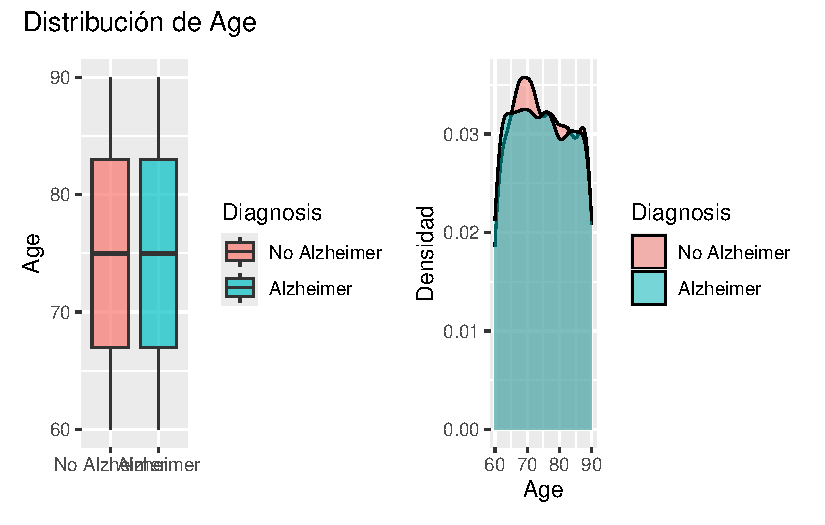
\includegraphics[width=0.9\linewidth,height=\textheight,keepaspectratio]{CATEDRA_1_ALZHEIMER_ML_files/figure-pdf/alzheimer_analisis-1.pdf}
\end{center}

\begin{verbatim}

--- Analizando: Gender vs Diagnosis ---
(Variable categórica)


Table: Gender vs Diagnosis

|Gender    | No Alzheimer| Alzheimer|
|:---------|------------:|---------:|
|Masculino |          675|       386|
|Femenino  |          714|       374|

Prueba Chi-cuadrado:

    Pearson's Chi-squared test with Yates' continuity correction

data:  datos[[col_nombre]] and datos[[var_objetivo]]
X-squared = 0.85972, df = 1, p-value = 0.3538

-> Sin asociación significativa (p >0.05)
\end{verbatim}

\begin{center}
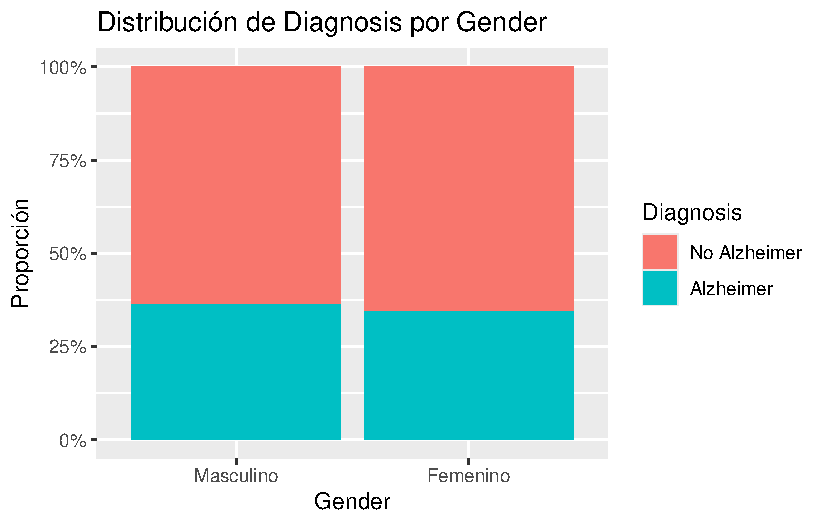
\includegraphics[width=0.9\linewidth,height=\textheight,keepaspectratio]{CATEDRA_1_ALZHEIMER_ML_files/figure-pdf/alzheimer_analisis-2.pdf}
\end{center}

\begin{verbatim}

--- Analizando: EducationLevel vs Diagnosis ---
(Variable categórica)


Table: EducationLevel vs Diagnosis

|EducationLevel | No Alzheimer| Alzheimer|
|:--------------|------------:|---------:|
|Ninguno        |          272|       174|
|Secundaria     |          552|       302|
|Universitario  |          419|       217|
|Superior       |          146|        67|

Prueba Chi-cuadrado:

    Pearson's Chi-squared test

data:  datos[[col_nombre]] and datos[[var_objetivo]]
X-squared = 4.4531, df = 3, p-value = 0.2165

-> Sin asociación significativa (p >0.05)
\end{verbatim}

\begin{center}
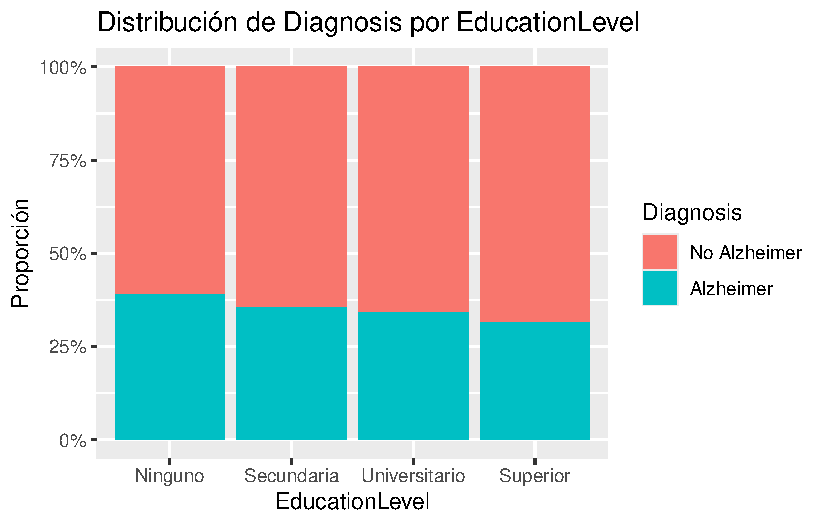
\includegraphics[width=0.9\linewidth,height=\textheight,keepaspectratio]{CATEDRA_1_ALZHEIMER_ML_files/figure-pdf/alzheimer_analisis-3.pdf}
\end{center}

\begin{verbatim}

--- Analizando: MMSE vs Diagnosis ---
(Variable numérica)


Table: Estadísticas de MMSE

|Diagnosis    |    n| Media|   SD|
|:------------|----:|-----:|----:|
|No Alzheimer | 1389| 16.27| 8.93|
|Alzheimer    |  760| 11.99| 7.23|

Prueba t-test (comparación de medias):

    Welch Two Sample t-test

data:  grupo1 and grupo2
t = 12.025, df = 1851.4, p-value < 2.2e-16
alternative hypothesis: true difference in means is not equal to 0
95 percent confidence interval:
 3.574302 4.967469
sample estimates:
mean of x mean of y 
 16.26554  11.99466 

-> Diferencias SIGNIFICATIVAS (p <0.05)
\end{verbatim}

\begin{center}
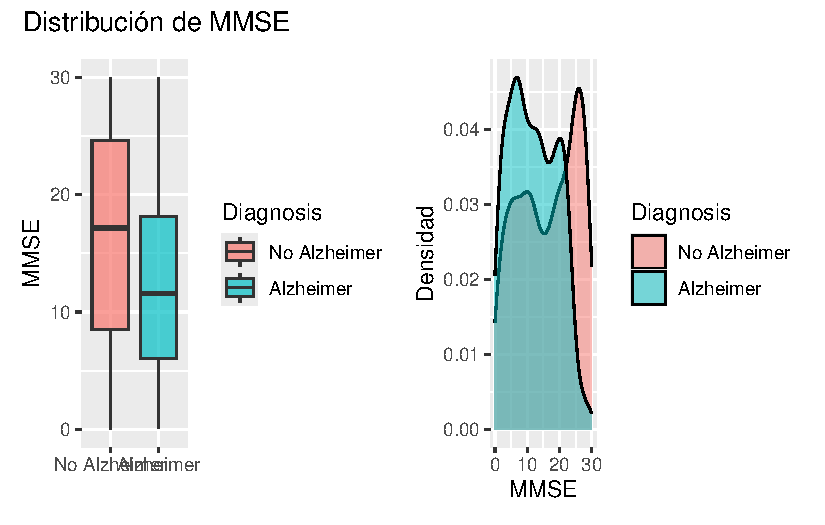
\includegraphics[width=0.9\linewidth,height=\textheight,keepaspectratio]{CATEDRA_1_ALZHEIMER_ML_files/figure-pdf/alzheimer_analisis-4.pdf}
\end{center}

\begin{verbatim}

--- Analizando: FamilyHistoryAlzheimers vs Diagnosis ---
(Variable categórica)


Table: FamilyHistoryAlzheimers vs Diagnosis

|FamilyHistoryAlzheimers | No Alzheimer| Alzheimer|
|:-----------------------|------------:|---------:|
|0                       |         1024|       583|
|1                       |          365|       177|

Prueba Chi-cuadrado:

    Pearson's Chi-squared test with Yates' continuity correction

data:  datos[[col_nombre]] and datos[[var_objetivo]]
X-squared = 2.1703, df = 1, p-value = 0.1407

-> Sin asociación significativa (p >0.05)
\end{verbatim}

\begin{center}
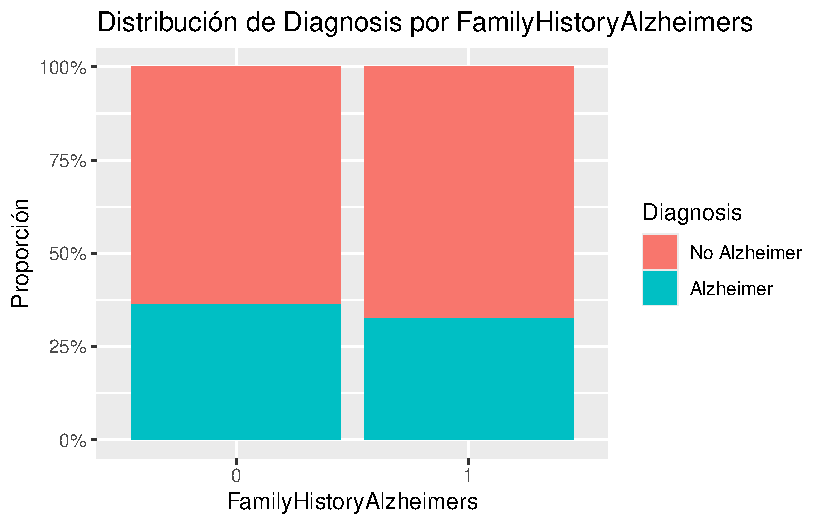
\includegraphics[width=0.9\linewidth,height=\textheight,keepaspectratio]{CATEDRA_1_ALZHEIMER_ML_files/figure-pdf/alzheimer_analisis-5.pdf}
\end{center}

\begin{verbatim}

--- Analizando: BMI vs Diagnosis ---
(Variable numérica)


Table: Estadísticas de BMI

|Diagnosis    |    n| Media|   SD|
|:------------|----:|-----:|----:|
|No Alzheimer | 1389| 27.52| 7.17|
|Alzheimer    |  760| 27.91| 7.30|

Prueba t-test (comparación de medias):

    Welch Two Sample t-test

data:  grupo1 and grupo2
t = -1.2148, df = 1537.9, p-value = 0.2246
alternative hypothesis: true difference in means is not equal to 0
95 percent confidence interval:
 -1.0395624  0.2444058
sample estimates:
mean of x mean of y 
 27.51509  27.91267 
\end{verbatim}

\begin{center}
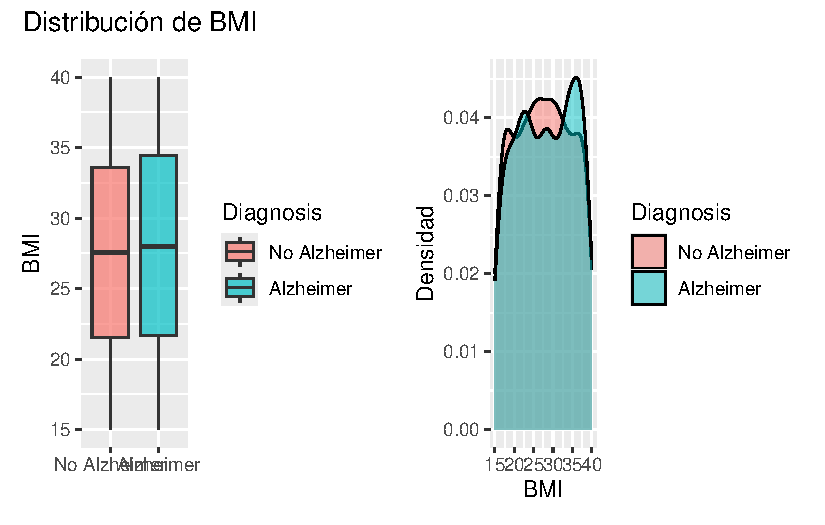
\includegraphics[width=0.9\linewidth,height=\textheight,keepaspectratio]{CATEDRA_1_ALZHEIMER_ML_files/figure-pdf/alzheimer_analisis-6.pdf}
\end{center}

\begin{verbatim}

--- Analizando: Smoking vs Diagnosis ---
(Variable categórica)


Table: Smoking vs Diagnosis

|Smoking | No Alzheimer| Alzheimer|
|:-------|------------:|---------:|
|0       |          986|       543|
|1       |          403|       217|

Prueba Chi-cuadrado:

    Pearson's Chi-squared test with Yates' continuity correction

data:  datos[[col_nombre]] and datos[[var_objetivo]]
X-squared = 0.030887, df = 1, p-value = 0.8605

-> Sin asociación significativa (p >0.05)
\end{verbatim}

\begin{center}
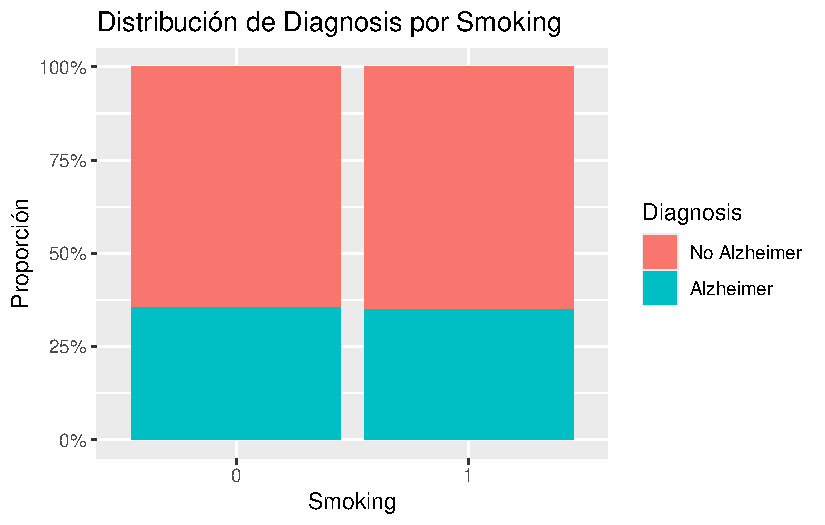
\includegraphics[width=0.9\linewidth,height=\textheight,keepaspectratio]{CATEDRA_1_ALZHEIMER_ML_files/figure-pdf/alzheimer_analisis-7.pdf}
\end{center}

\begin{verbatim}

--- Analizando: AlcoholConsumption vs Diagnosis ---
(Variable numérica)


Table: Estadísticas de AlcoholConsumption

|Diagnosis    |    n| Media|   SD|
|:------------|----:|-----:|----:|
|No Alzheimer | 1389| 10.07| 5.75|
|Alzheimer    |  760|  9.98| 5.77|

Prueba t-test (comparación de medias):

    Welch Two Sample t-test

data:  grupo1 and grupo2
t = 0.35271, df = 1557.6, p-value = 0.7244
alternative hypothesis: true difference in means is not equal to 0
95 percent confidence interval:
 -0.4183697  0.6018170
sample estimates:
mean of x mean of y 
10.071880  9.980156 
\end{verbatim}

\begin{center}
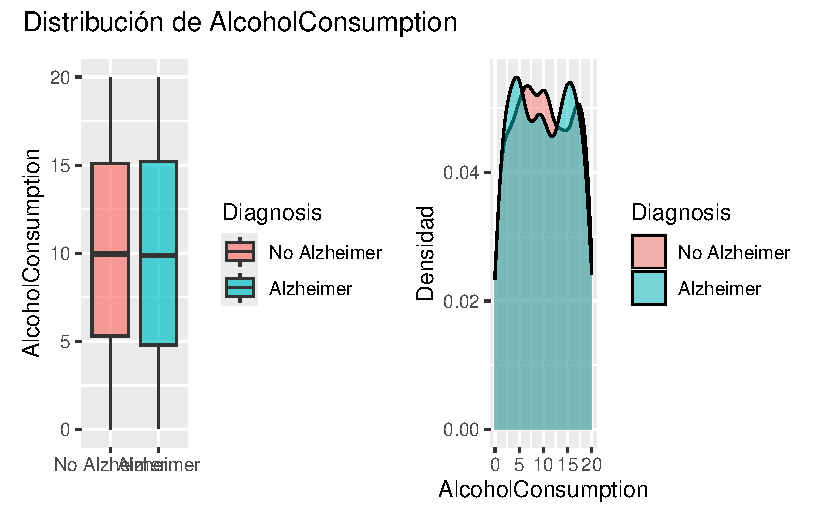
\includegraphics[width=0.9\linewidth,height=\textheight,keepaspectratio]{CATEDRA_1_ALZHEIMER_ML_files/figure-pdf/alzheimer_analisis-8.pdf}
\end{center}

\begin{verbatim}

--- Analizando: PhysicalActivity vs Diagnosis ---
(Variable numérica)


Table: Estadísticas de PhysicalActivity

|Diagnosis    |    n| Media|   SD|
|:------------|----:|-----:|----:|
|No Alzheimer | 1389|  4.91| 2.87|
|Alzheimer    |  760|  4.94| 2.84|

Prueba t-test (comparación de medias):

    Welch Two Sample t-test

data:  grupo1 and grupo2
t = -0.27642, df = 1576.9, p-value = 0.7823
alternative hypothesis: true difference in means is not equal to 0
95 percent confidence interval:
 -0.2875644  0.2165246
sample estimates:
mean of x mean of y 
  4.90764   4.94316 
\end{verbatim}

\begin{center}
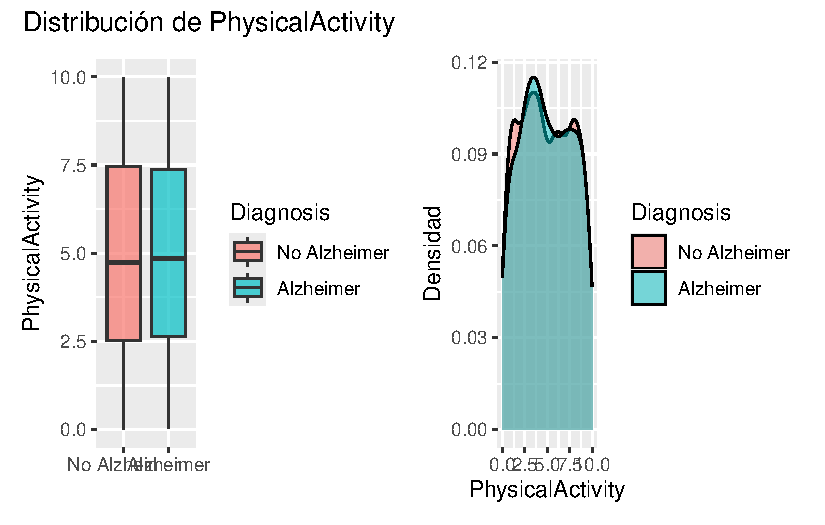
\includegraphics[width=0.9\linewidth,height=\textheight,keepaspectratio]{CATEDRA_1_ALZHEIMER_ML_files/figure-pdf/alzheimer_analisis-9.pdf}
\end{center}

\begin{verbatim}

--- Analizando: DietQuality vs Diagnosis ---
(Variable numérica)


Table: Estadísticas de DietQuality

|Diagnosis    |    n| Media|   SD|
|:------------|----:|-----:|----:|
|No Alzheimer | 1389|  4.97| 2.91|
|Alzheimer    |  760|  5.03| 2.91|

Prueba t-test (comparación de medias):

    Welch Two Sample t-test

data:  grupo1 and grupo2
t = -0.39404, df = 1560.2, p-value = 0.6936
alternative hypothesis: true difference in means is not equal to 0
95 percent confidence interval:
 -0.3093057  0.2058217
sample estimates:
mean of x mean of y 
 4.974839  5.026581 
\end{verbatim}

\begin{center}
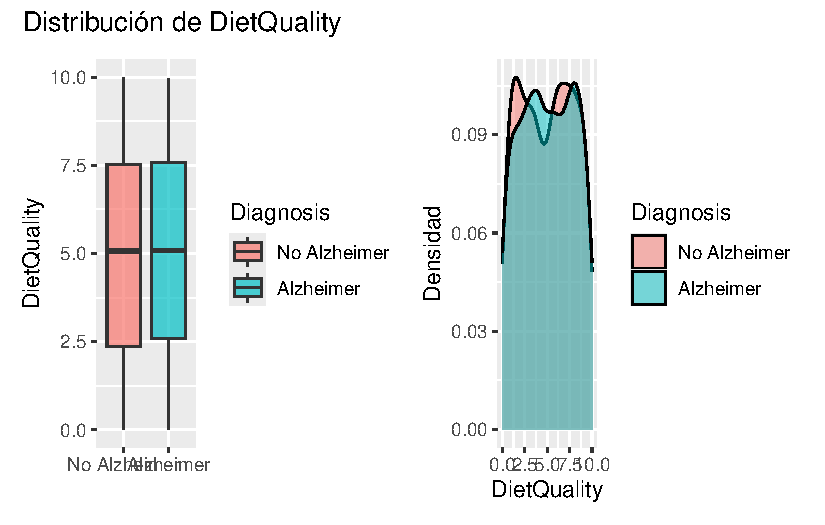
\includegraphics[width=0.9\linewidth,height=\textheight,keepaspectratio]{CATEDRA_1_ALZHEIMER_ML_files/figure-pdf/alzheimer_analisis-10.pdf}
\end{center}

\begin{verbatim}

--- Analizando: SleepQuality vs Diagnosis ---
(Variable numérica)


Table: Estadísticas de SleepQuality

|Diagnosis    |    n| Media|   SD|
|:------------|----:|-----:|----:|
|No Alzheimer | 1389|  7.12| 1.76|
|Alzheimer    |  760|  6.92| 1.76|

Prueba t-test (comparación de medias):

    Welch Two Sample t-test

data:  grupo1 and grupo2
t = 2.6282, df = 1567.7, p-value = 0.008669
alternative hypothesis: true difference in means is not equal to 0
95 percent confidence interval:
 0.05289963 0.36417980
sample estimates:
mean of x mean of y 
 7.124832  6.916292 

-> Diferencias SIGNIFICATIVAS (p <0.05)
\end{verbatim}

\begin{center}
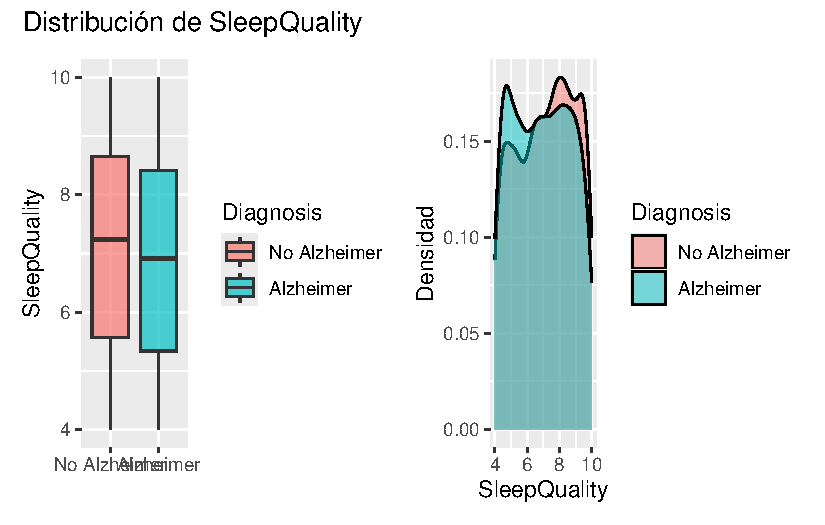
\includegraphics[width=0.9\linewidth,height=\textheight,keepaspectratio]{CATEDRA_1_ALZHEIMER_ML_files/figure-pdf/alzheimer_analisis-11.pdf}
\end{center}

\begin{verbatim}

--- Analizando: SystolicBP vs Diagnosis ---
(Variable numérica)


Table: Estadísticas de SystolicBP

|Diagnosis    |    n|  Media|    SD|
|:------------|----:|------:|-----:|
|No Alzheimer | 1389| 134.56| 25.95|
|Alzheimer    |  760| 133.72| 25.96|

Prueba t-test (comparación de medias):

    Welch Two Sample t-test

data:  grupo1 and grupo2
t = 0.7235, df = 1560.4, p-value = 0.4695
alternative hypothesis: true difference in means is not equal to 0
95 percent confidence interval:
 -1.449881  3.144540
sample estimates:
mean of x mean of y 
 134.5644  133.7171 
\end{verbatim}

\begin{center}
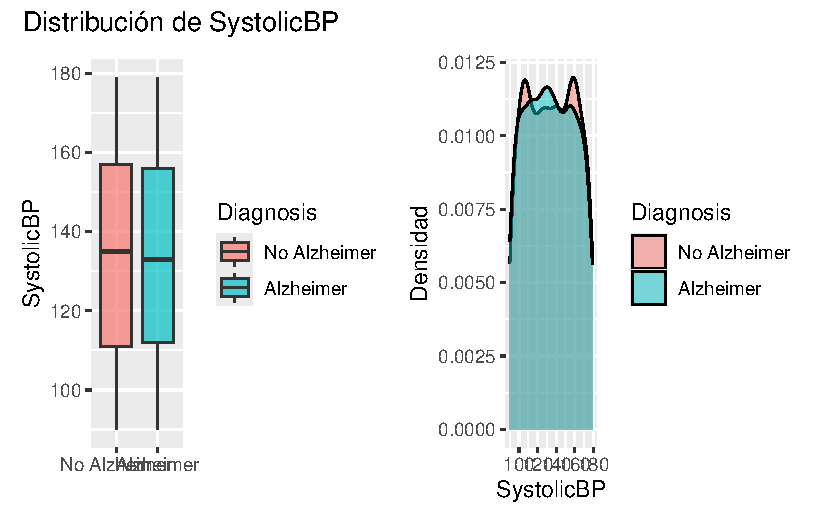
\includegraphics[width=0.9\linewidth,height=\textheight,keepaspectratio]{CATEDRA_1_ALZHEIMER_ML_files/figure-pdf/alzheimer_analisis-12.pdf}
\end{center}

\begin{verbatim}

--- Analizando: CholesterolTotal vs Diagnosis ---
(Variable numérica)


Table: Estadísticas de CholesterolTotal

|Diagnosis    |    n|  Media|    SD|
|:------------|----:|------:|-----:|
|No Alzheimer | 1389| 225.00| 42.20|
|Alzheimer    |  760| 225.57| 43.19|

Prueba t-test (comparación de medias):

    Welch Two Sample t-test

data:  grupo1 and grupo2
t = -0.29428, df = 1530.5, p-value = 0.7686
alternative hypothesis: true difference in means is not equal to 0
95 percent confidence interval:
 -4.360517  3.222806
sample estimates:
mean of x mean of y 
 224.9963  225.5652 
\end{verbatim}

\begin{center}
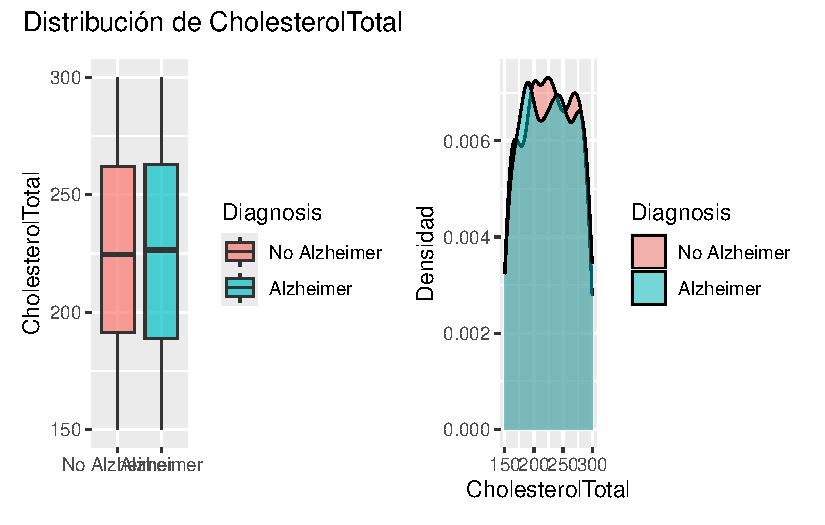
\includegraphics[width=0.9\linewidth,height=\textheight,keepaspectratio]{CATEDRA_1_ALZHEIMER_ML_files/figure-pdf/alzheimer_analisis-13.pdf}
\end{center}

\begin{verbatim}

--- Analizando: FunctionalAssessment vs Diagnosis ---
(Variable numérica)


Table: Estadísticas de FunctionalAssessment

|Diagnosis    |    n| Media|   SD|
|:------------|----:|-----:|----:|
|No Alzheimer | 1389|  5.86| 2.76|
|Alzheimer    |  760|  3.65| 2.57|

Prueba t-test (comparación de medias):

    Welch Two Sample t-test

data:  grupo1 and grupo2
t = 18.552, df = 1660.4, p-value < 2.2e-16
alternative hypothesis: true difference in means is not equal to 0
95 percent confidence interval:
 1.973921 2.440657
sample estimates:
mean of x mean of y 
 5.860669  3.653380 

-> Diferencias SIGNIFICATIVAS (p <0.05)
\end{verbatim}

\begin{center}
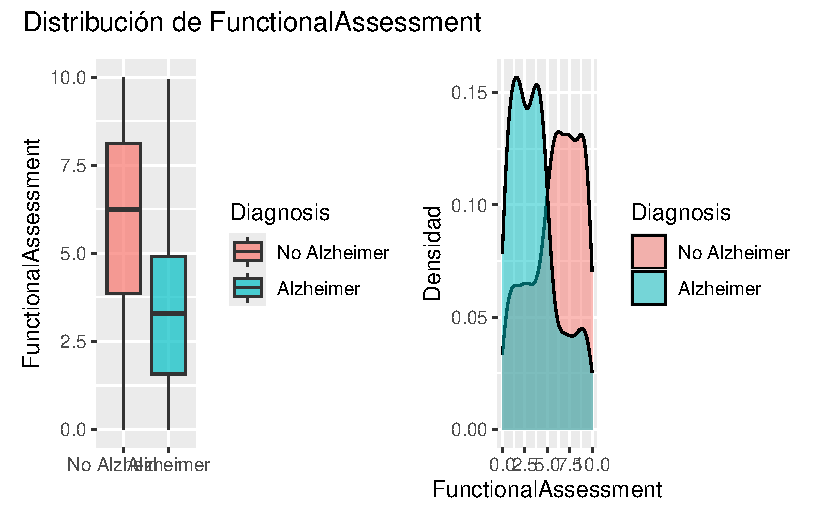
\includegraphics[width=0.9\linewidth,height=\textheight,keepaspectratio]{CATEDRA_1_ALZHEIMER_ML_files/figure-pdf/alzheimer_analisis-14.pdf}
\end{center}

\begin{verbatim}

--- Analizando: MemoryComplaints vs Diagnosis ---
(Variable categórica)


Table: MemoryComplaints vs Diagnosis

|MemoryComplaints | No Alzheimer| Alzheimer|
|:----------------|------------:|---------:|
|0                |         1228|       474|
|1                |          161|       286|

Prueba Chi-cuadrado:

    Pearson's Chi-squared test with Yates' continuity correction

data:  datos[[col_nombre]] and datos[[var_objetivo]]
X-squared = 200.62, df = 1, p-value < 2.2e-16

-> Asociación SIGNIFICATIVA (p <0.05)
\end{verbatim}

\begin{center}
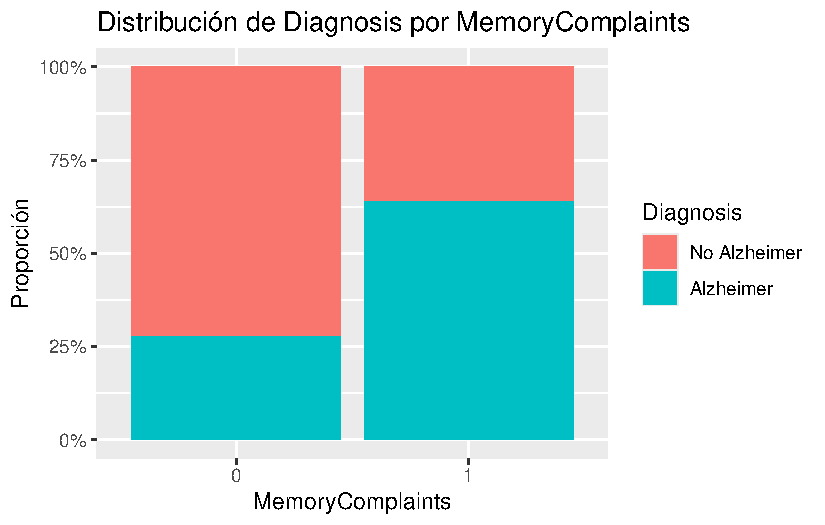
\includegraphics[width=0.9\linewidth,height=\textheight,keepaspectratio]{CATEDRA_1_ALZHEIMER_ML_files/figure-pdf/alzheimer_analisis-15.pdf}
\end{center}

\begin{verbatim}

--- Analizando: ADL vs Diagnosis ---
(Variable numérica)


Table: Estadísticas de ADL

|Diagnosis    |    n| Media|   SD|
|:------------|----:|-----:|----:|
|No Alzheimer | 1389|  5.71| 2.83|
|Alzheimer    |  760|  3.66| 2.70|

Prueba t-test (comparación de medias):

    Welch Two Sample t-test

data:  grupo1 and grupo2
t = 16.546, df = 1622.6, p-value < 2.2e-16
alternative hypothesis: true difference in means is not equal to 0
95 percent confidence interval:
 1.807000 2.293026
sample estimates:
mean of x mean of y 
 5.707951  3.657938 

-> Diferencias SIGNIFICATIVAS (p <0.05)
\end{verbatim}

\begin{center}
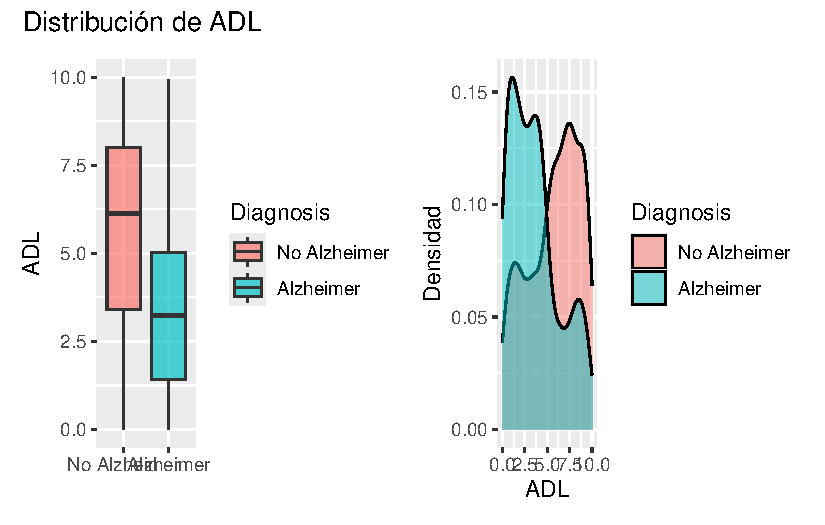
\includegraphics[width=0.9\linewidth,height=\textheight,keepaspectratio]{CATEDRA_1_ALZHEIMER_ML_files/figure-pdf/alzheimer_analisis-16.pdf}
\end{center}

\begin{verbatim}
-- FIN DEL ANÁLISIS EXPLORATORIO BIVARIADO ------------------------------------- 
\end{verbatim}

\section{Regresión logistica}\label{regresiuxf3n-logistica}

(desarrollo futuro)

\section{Machine learnig (ML)}\label{machine-learnig-ml}

(desarrollo futuro)

\section{\texorpdfstring{\textbf{Hallazgos
Principales}}{Hallazgos Principales}}\label{hallazgos-principales}

\begin{enumerate}
\def\labelenumi{\arabic{enumi}.}
\item
  \textbf{Relaciones significativas identificadas}:

  \begin{itemize}
  \item
    El análisis exploratorio bivariado reveló asociaciones
    estadísticamente significativas entre el diagnóstico de Alzheimer y
    variables como la edad, puntuaciones MMSE, antecedentes familiares y
    nivel educativo.
  \item
    Las pruebas estadísticas (chi-cuadrado, t-test) confirmaron estas
    relaciones con valores p significativos.
  \end{itemize}
\item
  \textbf{Variables predictoras clave}:

  \begin{itemize}
  \item
    \textbf{Edad}: Confirmada como factor de riesgo importante, con
    pacientes mayores mostrando mayor prevalencia de Alzheimer.
  \item
    \textbf{MMSE}: Puntuaciones más bajas se asociaron fuertemente con
    diagnóstico positivo.
  \item
    \textbf{Antecedentes familiares}: Variable categórica con impacto
    significativo en el diagnóstico.
  \item
    \textbf{Nivel educativo}: Se observó un efecto protector de mayor
    educación.
  \end{itemize}
\item
  \textbf{Calidad de datos}:

  \begin{itemize}
  \tightlist
  \item
    Las transformaciones de variables (especialmente a factores
    ordenados) permitieron análisis más robustos.
  \end{itemize}
\end{enumerate}

\subsection{\texorpdfstring{\textbf{Limitaciones}}{Limitaciones}}\label{limitaciones}

\begin{enumerate}
\def\labelenumi{\arabic{enumi}.}
\item
  El análisis se basó en datos secundarios con limitaciones en el tamaño
  muestral y variables disponibles.
\item
  El estudio es observacional, por lo que no se pueden establecer
  relaciones causales.
\item
  El modelo predictivo (regresión logística) mencionado como desarrollo
  futuro requeriría validación adicional.
\end{enumerate}

\subsection{\texorpdfstring{\textbf{Recomendaciones}}{Recomendaciones}}\label{recomendaciones}

\begin{enumerate}
\def\labelenumi{\arabic{enumi}.}
\item
  \textbf{Para mi investigación futura}:

  \begin{itemize}
  \item
    Implementar los modelos predictivos propuestos (regresión logística
    y machine learning).
  \item
    Considerar interacciones entre variables en análisis multivariados.
  \item
    Validar los hallazgos con muestras independientes.
  \end{itemize}
\end{enumerate}

\subsection{\texorpdfstring{\textbf{Conclusión
Final}}{Conclusión Final}}\label{conclusiuxf3n-final}

Este análisis proporciona evidencia estadística sólida sobre los
factores asociados al diagnóstico de Alzheimer, destacando la utilidad
del enfoque Tidyverse para el procesamiento y exploración de datos
médicos. Los hallazgos sientan las bases para el desarrollo futuro de
modelos predictivos que podrían contribuir a la detección temprana de
esta condición neurodegenerativa.




\end{document}
